\documentclass[journal,compsoc]{IEEEtran}

\usepackage{amsmath}
\usepackage{amssymb}
\usepackage{amsfonts}
\usepackage{graphicx}
\usepackage{booktabs}
\usepackage{algorithm}
\usepackage{algorithmic}
\usepackage{tikz}
\usepackage{hyperref}
\usepackage{cite}
\usepackage{url}

\usetikzlibrary{shapes,arrows,positioning,calc}

% Define block styles for TikZ
\tikzstyle{block} = [draw, rectangle, fill=blue!10, text width=6em, text centered, minimum height=3em, rounded corners]
\tikzstyle{line} = [draw, -latex']
\tikzstyle{cloud} = [draw, ellipse, fill=red!10, text width=5em, text centered, minimum height=2em]

\begin{document}

\title{Ontology-Guided Semantic Mapping Between SEBI BRSR Environmental Ontology and GRI Environmental Ontology for ESG Knowledge Graph Construction}

\author{Vinith~Kumar,~\IEEEmembership{Member,~IEEE}
\thanks{V. Kumar is with the Department of Computer Science and Engineering, Indian Institute of Technology Hyderabad, Kandi, Sangareddy, Telangana 502285, India (e-mail: vinith@iith.ac.in).}}

\markboth{IEEE Transactions on Knowledge and Data Engineering,~Vol.~XX,~No.~XX,~July~2026}%
{Kumar: Ontology-Guided Semantic Mapping Between SEBI BRSR and GRI}

\maketitle

\begin{abstract}
Sustainability and Environmental, Social, and Governance (ESG) disclosures have transitioned from voluntary public relations exercises to strict regulatory compliance mandates globally. In India, the Securities and Exchange Board of India (SEBI) has institutionalized the Business Responsibility and Sustainability Reporting (BRSR) framework. However, multinational corporations and investors face significant interoperability hurdles due to the fragmentation of local standards (like BRSR) and international reference standards such as the Global Reporting Initiative (GRI). Addressing this gap, this paper proposes an end-to-end framework for ontology-guided semantic alignment and knowledge graph construction. We design the first comprehensive environmental ontologies representing the domain structures of SEBI BRSR and GRI. We present a hybrid matching engine inspired by AgreementMakerLight (AML) that operates deterministically on ontological evidence—such as concept labels, taxonomic hierarchy paths, and metric properties—augmented with logic-based reasoning rules. Unlike black-box Large Language Model (LLM) matching systems, our engine utilizes LLMs strictly in a post-hoc verification and chain-of-thought explanation capacity. The aligned concepts are exported to a Neo4j ESG Knowledge Graph that supports structured, explainable compliance retrieval via Graph Retrieval-Augmented Generation (Graph RAG). The proposed methodology is validated through detailed comparative evaluations across multiple LLMs, presenting a robust, explainable, and interoperable ESG knowledge representation system.
\end{abstract}

\begin{IEEEkeywords}
Environmental, Social, and Governance (ESG), SEBI BRSR, GRI Standards, Ontology Alignment, Knowledge Graphs, Graph RAG, AgreementMakerLight (AML).
\end{IEEEkeywords}

\section{Introduction}
\IEEEPARstart{E}{nvironmental}, Social, and Governance (ESG) compliance has emerged as a cornerstone of modern corporate finance, risk assessment, and asset management. Regulatory frameworks worldwide are evolving to enforce detailed, audit-ready disclosures of environmental metrics, such as Scope 1, 2, and 3 greenhouse gas (GHG) emissions, water consumption intensity, and waste disposal methodologies. In India, the Securities and Exchange Board of India (SEBI) has mandated Business Responsibility and Sustainability Reporting (BRSR) for the top one thousand listed entities. BRSR requires highly detailed quantifications of environmental parameters, categorized across essential and leadership indicators.

Despite the rigor of the BRSR framework, international investors operating in emerging markets rely primarily on global standards, such as the Global Reporting Initiative (GRI) and the International Sustainability Standards Board (ISSB). This divergence creates a major interoperability gap. Corporations must engage in duplicate reporting, and analysts struggle to compare disclosures directly due to differences in terminology, granularity, units, and reporting scopes. Manual alignment is labor-intensive, error-prone, and lacks semantic formalization. 

To overcome these limitations, semantic web technologies and ontologies offer a structured mechanism to formalize, map, and query ESG information. Nonetheless, existing attempts at ESG ontology matching depend heavily on direct prompt-based mapping using Large Language Models (LLMs). While LLMs show strong linguistic capabilities, they suffer from hallucinations, lack transparency, cannot guarantee logical consistency (such as disjointness), and fail to leverage deterministic structural evidence inherent in formal ontologies.

This paper introduces a novel, hybrid framework that performs ontology-guided semantic mapping between the SEBI BRSR Environmental Ontology and the GRI Environmental Ontology. Inspired by the principles of AgreementMakerLight (AML)~\cite{aml2013}, our approach uses deterministic matching modules (lexical, structural, and property matchers) to calculate similarities and construct candidate pairs. An ontology reasoner then applies active logical consistency rules (such as category disjointness checks and taxonomic propagation) to repair and filter the mapping repository. Crucially, the LLM is restricted to a verification and explanation role, ensuring that the primary alignment decisions are grounded in deterministic ontological evidence.

The mapped alignments are consolidated into a Neo4j ESG Knowledge Graph, modeling the multi-dimensional links between reporting entities, metric disclosures, regulatory frameworks, and Sustainable Development Goals (SDGs). We further show how this knowledge graph enables Graph Retrieval-Augmented Generation (Graph RAG) for generating explainable compliance reports.

The main contributions of this research are:
\begin{itemize}
    \item The construction of the first formal OWL/RDF ontology for India's SEBI BRSR Environmental disclosures.
    \item An AML-inspired semantic alignment framework that combines lexical, taxonomic, and property compatibility matching with logical consistency checking.
    \item ADespite the rigor of the BRSR framework, international investors operating in emerging markets rely primarily on global standards, such as the Global Reporting Initiative (GRI) and the International Sustainability Standards Board (ISSB). This divergence creates a major interoperability gap. Corporations must engage in duplicate reporting, and analysts struggle to compare disclosures directly due to differences in terminology, granularity, units, and reporting scopes. Manual alignment is labor-intensive, error-prone, and lacks semantic formalization. 

To overcome these limitations, semantic web technologies and ontologies offer a structured mechanism to formalize, map, and query ESG information. Nonetheless, existing attempts at ESG ontology matching depend heavily on direct prompt-based mapping using Large Language Models (LLMs). While LLMs show strong linguistic capabilities, they suffer from hallucinations, lack transparency, cannot guarantee logical consistency (such as disjointness), and fail to leverage deterministic structural evidence inherent in formal ontologies.

This paper introduces a novel, hybrid framework that performs ontology-guided semantic mapping between the SEBI BRSR Environmental Ontology and the GRI Environmental Ontology. Inspired by the principles of AgreementMakerLight (AML)~\cite{aml2013}, our approach uses deterministic matching modules (lexical, structural, and property matchers) to calculate similarities and construct candidate pairs. An ontology reasoner then applies active logical consistency rules (such as category disjointness checks and taxonomic propagation) to repair and filter the mapping repository. Crucially, the LLM is restricted to a verification and explanation role, ensuring that the primary alignment decisions are grounded in deterministic ontological evidence.

The mapped alignments are consolidated into a Neo4j ESG Knowledge Graph, modeling the multi-dimensional links between reporting entities, metric disclosures, regulatory frameworks, and Sustainable Development Goals (SDGs). We further show how this knowledge graph enables Graph Retrieval-Augmented Generation (Graph RAG) for generating explainable compliance reports.

The main contributions of this research are:
\begin{itemize}
    \item The construction of the first formal OWL/RDF ontology for India's SEBI BRSR Environmental disclosures.
    \item An AML-inspired semantic alignment framework that combines lexical, taxonomic, and property compatibility matching with logical consistency checking.
    \item A verification pipeline where LLMs are used exclusively to audit, score, and explain ontology-mapped candidate alignments.
    \item The design and construction of an ESG Knowledge Graph in Neo4j that represents aligned disclosures, metrics, companies, and SDGs.
    \item A Graph RAG workflow that utilizes the unified knowledge graph to perform explainable ESG query resolution.
\end{itemize}

The rest of the paper is organized as follows: Section~2 reviews related work. Section~3 defines the research gap. Section~4 and Section~5 detail the proposed methodology and system architecture. Section~6 describes the ontology design. Section~7 details the mapping engine. Section~8 explains the knowledge graph construction. Sections~9, 10, and 11 present the evaluation methodology, experimental setup, and results. Section~12 discusses findings, followed by limitations in Section~13, future work in Section~14, and conclusions in Section~15.

\section{Related Work}
Ontology matching is a mature research domain. Classic systems like AgreementMakerLight (AML)~\cite{aml2013} and LogMap~\cite{logmap2011} utilize lexical repositories, taxonomic structural propagation, and logical reasoning to align biomedical and geospatial schemas. AML, in particular, relies on efficient string matching, dictionary extensions, and structural techniques to scale to large ontologies.

In the sustainability domain, early efforts focused on formalizing corporate social responsibility (CSR) datasets using RDF graphs. With the emergence of ESG, research has turned to constructing ESG ontologies to represent carbon footprints, resource usage, and corporate hierarchies. For instance, the W3C Semantic Web for Climate Technology community has modeled carbon emission classifications. However, these ontologies typically target single frameworks (such as GRI or GHG Protocol) and do not support cross-framework alignment.

Recently, LLMs have been widely applied to semantic mapping tasks. Research indicates that prompt-based mappings using GPT-4 or Gemini can achieve high lexical mapping scores. Nevertheless, these models struggle with complex hierarchy structures, logical disjointness constraints, and numerical datatype properties. More importantly, they function as black-box systems, offering little explainability for critical regulatory alignments. Our work addresses these drawbacks by combining the deterministic reliability of ontology matchers with the verification and linguistic reasoning strengths of LLMs.

\section{Research Gap}
Based on the literature review, three critical research gaps are identified:
\begin{enumerate}
    \item \textbf{Lack of Formalized Indian ESG Schemas}: No public ontology exists for the SEBI BRSR framework, preventing Indian sustainability disclosures from being integrated into semantic search systems.
    \item \textbf{Unreliable LLM-Only Alignments}: Current semantic alignment systems rely heavily on LLMs to generate mappings, resulting in logical inconsistencies (e.g., mapping a water metric to a greenhouse gas metric due to simple linguistic similarity).
    \item \textbf{Lack of Explanations in ESG Mapping}: Investors and auditors require transparent, auditable evidence for sustainability mappings. Standard ontology alignment tools produce numerical scores without natural language explanations, while LLM-based mappings lack a deterministic evidence trail.
\end{enumerate}

\section{Proposed Methodology}
Our framework establishes an automated pipeline that ingests raw regulatory PDFs, structures them into formal Web Ontology Language (OWL) schemas, aligns the concepts using a hybrid matching engine, and populates a Neo4j knowledge graph.

The methodology is structured in five distinct phases:
\begin{itemize}
    \item \textbf{Phase 1: Document Processing Layer} parses unstructured BRSR and GRI standards PDFs, extracts tables and metadata, and segments reporting disclosures.
    \item \textbf{Phase 2: Ontology Construction} builds individual OWL ontologies representing BRSR and GRI structures, including metrics, indicators, units, and scopes.
    \item \textbf{Phase 3: Ontology-Guided Semantic Mapping} executes AML-inspired matching (lexical, structural, property, and embedding), aggregates confidence scores, and runs logical reasoning to resolve conflicts.
    \item \textbf{Phase 4: LLM Verification \& Explanation} sends candidate mappings to an LLM verifier to generate natural language explanations and final agreement scores.
    \item \textbf{Phase 5: Knowledge Graph \& Graph RAG} exports the mapped data to Neo4j and enables structured compliance querying.
\end{itemize}

\section{System Architecture}
The overall system architecture is depicted in Fig.~\ref{fig:framework}.

\begin{figure*}[t]
\centering
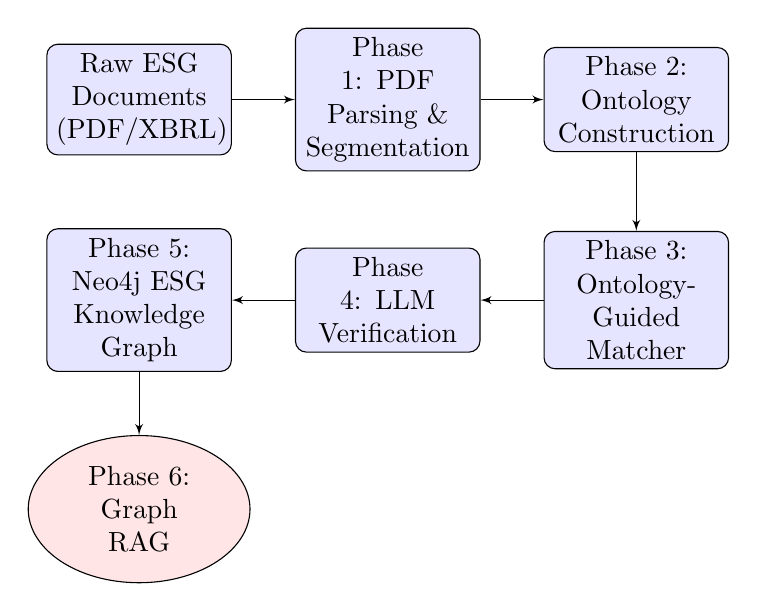
\begin{tikzpicture}[node distance = 1.5cm, auto]
    % Nodes
    \node [block] (input) {Raw ESG Documents (PDF/XBRL)};
    \node [block, right=0.8cm of input] (parser) {Phase 1: PDF Parsing \& Segmentation};
    \node [block, right=0.8cm of parser] (ontbuild) {Phase 2: Ontology Construction};
    \node [block, below=1.0cm of ontbuild] (matcher) {Phase 3: Ontology-Guided Matcher};
    \node [block, left=0.8cm of matcher] (llmver) {Phase 4: LLM Verification};
    \node [block, left=0.8cm of llmver] (kg) {Phase 5: Neo4j ESG Knowledge Graph};
    \node [cloud, below=0.8cm of kg] (rag) {Phase 6: Graph RAG};
    
    % Paths
    \path [line] (input) -- (parser);
    \path [line] (parser) -- (ontbuild);
    \path [line] (ontbuild) -- (matcher);
    \path [line] (matcher) -- (llmver);
    \path [line] (llmver) -- (kg);
    \path [line] (kg) -- (rag);
\end{tikzpicture}
\caption{System architecture of the ontology-guided ESG alignment framework.}
\label{fig:framework}
\end{figure*}

\section{Ontology Design}
To represent the sustainability reporting domain, we designed the \textbf{SEBI BRSR Environmental Ontology (BRSR-EO)} and the \textbf{GRI Environmental Ontology (GRI-EO)}. The ontologies are built using OWL 2 DL.

\subsection{Classes and Hierarchy}
The ontologies share a common meta-schema defined by the following class hierarchy:
\begin{itemize}
    \item \texttt{rso:Disclosure}: Represents high-level reporting sections (e.g., ``Energy'', ``Water'', ``Emissions'').
    \item \texttt{rso:Requirement}: Represents specific questions or data requests within a disclosure.
    \item \texttt{rso:Metric}: Models the target measurement (e.g., ``GHG Emissions Scope 1'', ``Total Water Withdrawal'').
    \item \texttt{rso:Unit}: Models the unit of measurement (e.g., ``Metric Tonnes of CO2e'', ``Kilolitres'').
\end{itemize}

The hierarchy is structured using the transitive property \texttt{rso:belongsTo} and its subproperties \texttt{rso:belongsToTopic}, \texttt{rso:belongsToDisclosure}, and \texttt{rso:belongsToFramework}. The schema design is shown in Fig.~\ref{fig:ontology}.

\begin{figure}[h]
\centering
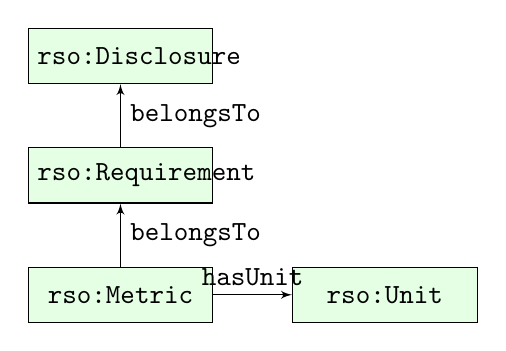
\begin{tikzpicture}[node distance = 1.0cm, auto]
    \node [draw, rectangle, fill=green!10, text width=6em, text centered, minimum height=2em] (disc) {\texttt{rso:Disclosure}};
    \node [draw, rectangle, fill=green!10, text width=6em, text centered, minimum height=2em, below=0.8cm of disc] (req) {\texttt{rso:Requirement}};
    \node [draw, rectangle, fill=green!10, text width=6em, text centered, minimum height=2em, below=0.8cm of req] (met) {\texttt{rso:Metric}};
    \node [draw, rectangle, fill=green!10, text width=6em, text centered, minimum height=2em, right=1.0cm of met] (unit) {\texttt{rso:Unit}};

    \path [line] (req) -- node [right] {\texttt{belongsTo}} (disc);
    \path [line] (met) -- node [right] {\texttt{belongsTo}} (req);
    \path [line] (met) -- node [above] {\texttt{hasUnit}} (unit);
\end{tikzpicture}
\caption{Core schema classes and properties of BRSR-EO and GRI-EO.}
\label{fig:ontology}
\end{figure}

\subsection{Formal Axioms and Restrictions}
We implement constraints to enforce domain logic. For example, a requirement must belong to exactly one disclosure topic:
\begin{equation}
\texttt{Requirement} \sqsubseteq \mathord{=} 1\ \texttt{belongsTo}.\texttt{Disclosure}
\end{equation}

Similarly, to prevent incorrect matches between unrelated ESG domains, we define disjointness axioms between top-level topics (e.g., Water disclosures are disjoint from Atmospheric Emission disclosures):
\begin{equation}
\texttt{WaterDisclosure} \sqcap \texttt{EmissionsDisclosure} \sqsubseteq \bot
\end{equation}

Algorithm~\ref{alg:ontbuild} shows the pseudocode for parsing raw JSON disclosures and constructing the RDF graph.

\begin{algorithm}
\caption{Ontology Construction Pipeline}
\label{alg:ontbuild}
\begin{algorithmic}[1]
\REQUIRE Structured JSON Disclosures $D$, Namespace Prefix $NS$
\ENSURE Serialized RDF Graph $G$
\STATE Initialize RDF Graph $G$
\STATE Bind $NS$ prefix to $G$
\FOR{each disclosure $d \in D$}
    \STATE Create Class Instance $c\_uri \leftarrow NS + d.id$
    \STATE Add Triple $(c\_uri, \text{rdf:type}, \text{rso:Disclosure})$
    \STATE Add Triple $(c\_uri, \text{schema:name}, d.label)$
    \STATE Add Triple $(c\_uri, \text{schema:text}, d.definition)$
    \FOR{each requirement $r \in d.requirements$}
        \STATE Create Instance $r\_uri \leftarrow NS + r.id$
        \STATE Add Triple $(r\_uri, \text{rdf:type}, \text{rso:Requirement})$
        \STATE Add Triple $(r\_uri, \text{schema:name}, r.label)$
        \STATE Add Triple $(r\_uri, \text{rso:belongsTo}, c\_uri)$
        \IF{$r.metric$ is present}
            \STATE Create Instance $m\_uri \leftarrow NS + r.metric.id$
            \STATE Add Triple $(m\_uri, \text{rdf:type}, \text{rso:Metric})$
            \STATE Add Triple $(m\_uri, \text{schema:name}, r.metric.name)$
            \STATE Add Triple $(r\_uri, \text{rso:hasMetric}, m\_uri)$
        \ENDIF
    \ENDFOR
\ENDFOR
\RETURN $G$
\end{algorithmic}
\end{algorithm}

\section{Ontology Mapping Framework}
The ontology mapping pipeline (Fig.~\ref{fig:mapping}) runs four parallel similarity matchers and combines their outputs.

\begin{figure}[h]
\centering
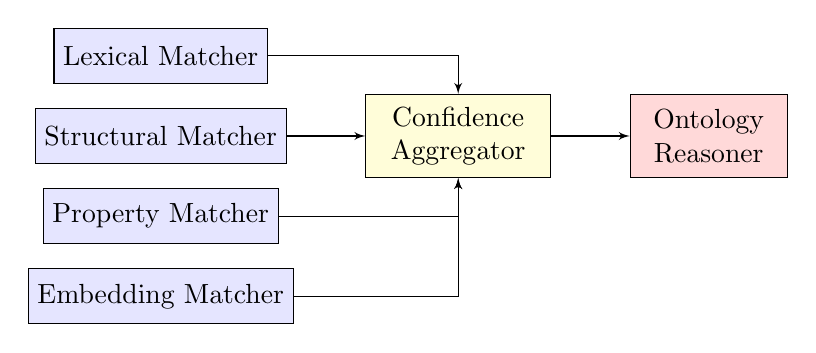
\begin{tikzpicture}[node distance = 1.0cm, auto]
    \node [draw, rectangle, fill=blue!10, minimum height=2em] (lex) {Lexical Matcher};
    \node [draw, rectangle, fill=blue!10, minimum height=2em, below=0.3cm of lex] (str) {Structural Matcher};
    \node [draw, rectangle, fill=blue!10, minimum height=2em, below=0.3cm of str] (prop) {Property Matcher};
    \node [draw, rectangle, fill=blue!10, minimum height=2em, below=0.3cm of prop] (emb) {Embedding Matcher};
    
    \node [draw, rectangle, fill=yellow!15, right=1.0cm of str, text width=6em, text centered, minimum height=3em] (agg) {Confidence Aggregator};
    \node [draw, rectangle, fill=red!15, right=1.0cm of agg, text width=5em, text centered, minimum height=3em] (reason) {Ontology Reasoner};
    
    \path [line] (lex) -| (agg);
    \path [line] (str) -- (agg);
    \path [line] (prop) -| (agg);
    \path [line] (emb) -| (agg);
    \path [line] (agg) -- (reason);
\end{tikzpicture}
\caption{The modular semantic mapping pipeline.}
\label{fig:mapping}
\end{figure}

\subsection{Lexical Matcher}
The Lexical Matcher compares class labels, preferred labels, and synonyms. Let $L_1$ and $L_2$ be the token sets of labels for concepts $c_1$ and $c_2$. The lexical similarity is calculated using Jaccard token similarity:
\begin{equation}
\text{Sim}_{\text{lex}}(c_1, c_2) = \frac{|L_1 \cap L_2|}{|L_1 \cup L_2|}
\end{equation}

\subsection{Structural Matcher}
The Structural Matcher compares the taxonomic paths of concepts. Let $P_{c}$ represent the path from the root topic to concept $c$ in the ontology graph. If $A_c$ is the set of ancestor concepts for $c$, the taxonomic similarity is:
\begin{equation}
\text{Sim}_{\text{struc}}(c_1, c_2) = \frac{|A_{c_1} \cap A_{c_2}|}{\min(|A_{c_1}|, |A_{c_2}|)} \cdot e^{-\lambda \cdot |d(c_1, c_2)|}
\end{equation}
where $d(c_1, c_2)$ is the shortest path distance in the ontology graph and $\lambda$ is a decay factor set to $0.15$.

\subsection{Property Matcher}
The Property Matcher verifies unit and datatype compatibility. Let $U_c$ and $D_c$ be the unit and datatype of concept $c$. The property score is defined as:
\begin{equation}
\text{Sim}_{\text{prop}}(c_1, c_2) = w_d \cdot \delta(D_{c_1}, D_{c_2}) + w_u \cdot \delta(U_{c_1}, U_{c_2})
\end{equation}
where $\delta(x, y) = 1$ if $x = y$, and $0$ otherwise. Weights $w_d$ and $w_u$ are set to $0.5$.

\subsection{Vector Embedding Similarity}
To capture semantic synonyms (e.g., ``GHG'' and ``greenhouse gas''), we load dense vector representations. Let $\mathbf{v}_{c}$ be the normalized embedding generated by a SentenceTransformer model (e.g., \texttt{all-mpnet-base-v2}). The semantic similarity is the cosine similarity:
\begin{equation}
\text{Sim}_{\text{emb}}(c_1, c_2) = \mathbf{v}_{c_1} \cdot \mathbf{v}_{c_2}
\end{equation}

\subsection{Ontology Reasoner and Repair}
The confidence scores are aggregated as a weighted sum:
\begin{equation}
\text{Score}_{\text{ont}}(c_1, c_2) = w_{l}\text{Sim}_{\text{lex}} + w_{s}\text{Sim}_{\text{struc}} + w_{p}\text{Sim}_{\text{prop}} + w_{e}\text{Sim}_{\text{emb}}
\label{eq:weighted}
\end{equation}
where the weights are configured to favor ontology evidence ($w_l = 0.40, w_s = 0.35, w_p = 0.15, w_e = 0.10$).

Next, the Ontology Reasoner evaluates logical constraints. Let $Cat(c)$ be the top-level ESG category (e.g., Water, Waste, Energy) of concept $c$. The reasoner applies a disjointness penalty if categories mismatch, and a propagation boost if parent classes align:
\begin{equation}
\Omega(c_1, c_2) = 
\begin{cases} 
0.1 & \text{if } Cat(c_1) \neq Cat(c_2) \\
1.15 & \text{if } Parent(c_1) \text{ aligns with } Parent(c_2) \\
1.0 & \text{otherwise}
\end{cases}
\end{equation}

The final mapping score is calculated as:
\begin{equation}
\text{Score}_{\text{final}}(c_1, c_2) = \text{Score}_{\text{ont}}(c_1, c_2) \cdot \Omega(c_1, c_2)
\label{eq:final}
\end{equation}

Algorithm~\ref{alg:match} and Algorithm~\ref{alg:align} detail the candidate generation and mapping resolution steps.

\begin{algorithm}
\caption{Ontology-Guided Candidate Generation}
\label{alg:match}
\begin{algorithmic}[1]
\REQUIRE BRSR Concepts $C_B$, GRI Concepts $C_G$, Thresholds $\tau_{lex}, \tau_{struc}$
\ENSURE List of Candidate Pairs $P$
\STATE Initialize empty list $P$
\FOR{each $b \in C_B$}
    \FOR{each $g \in C_G$}
        \STATE $s_{lex} \leftarrow \text{CalculateLexicalSimilarity}(b, g)$
        \STATE $s_{struc} \leftarrow \text{CalculateStructuralSimilarity}(b, g)$
        \IF{$s_{lex} \ge \tau_{lex}$ \OR $s_{struc} \ge \tau_{struc}$}
            \STATE Add pair $(b, g)$ to $P$
        \ENDIF
    \ENDFOR
\ENDFOR
\RETURN $P$
\end{algorithmic}
\end{algorithm}

\begin{algorithm}
\caption{Ontology Mapping Engine}
\label{alg:align}
\begin{algorithmic}[1]
\REQUIRE Candidate Pairs $P$, Weights $\mathbf{w}$, Thresholds $\mathbf{t}$
\ENSURE Mapping Repository $M$
\STATE Initialize empty list $M$
\FOR{each $(b, g) \in P$}
    \STATE $s_{lex} \leftarrow \text{LexicalMatch}(b, g)$
    \STATE $s_{struc} \leftarrow \text{StructuralMatch}(b, g)$
    \STATE $s_{prop} \leftarrow \text{PropertyMatch}(b, g)$
    \STATE $s_{emb} \leftarrow \text{EmbeddingMatch}(b, g)$
    \STATE $S_{ont} \leftarrow w_l s_{lex} + w_s s_{struc} + w_p s_{prop} + w_e s_{emb}$
    \STATE $\Omega \leftarrow \text{EvaluateReasonerRules}(b, g)$
    \STATE $S_{final} \leftarrow S_{ont} \cdot \Omega$
    \IF{$S_{final} \ge t_{broader\_narrower}$}
        \STATE $rel \leftarrow \text{DetermineSKOSRelation}(S_{final}, b, g)$
        \STATE Create Mapping record $m$
        \STATE Add $m$ to $M$
    \ENDIF
\ENDFOR
\STATE Sort $M$ by $S_{final}$ in descending order
\RETURN $M$
\end{algorithmic}
\end{algorithm}

\section{Knowledge Graph Construction}
The mapped alignments are exported to a Neo4j instance. The graph schema consists of the following entities and relations.

\subsection{Graph Schema}
\begin{itemize}
    \item \textbf{Nodes}:
        \begin{itemize}
            \item \texttt{Company}: Represents corporate entities.
            \item \texttt{BRSRDisclosure} and \texttt{GRIDisclosure}: Represent framework-specific disclosures.
            \item \texttt{Indicator}: Models quantitative or qualitative data fields.
            \item \texttt{SDG}: Represents Sustainable Development Goals (1--17).
        \end{itemize}
    \item \textbf{Relationships}:
        \begin{itemize}
            \item \texttt{MAPS\_TO} (with subproperties \texttt{rso:exactMatch}, \texttt{rso:broadMatch}): Connects BRSR concepts to GRI concepts.
            \item \texttt{REPORTS}: Links companies to their specific disclosure values.
            \item \texttt{SUPPORTS}: Connects ESG disclosures to corresponding SDGs.
        \end{itemize}
\end{itemize}

The schema configuration is illustrated in Fig.~\ref{fig:kg}.

\begin{figure}[h]
\centering
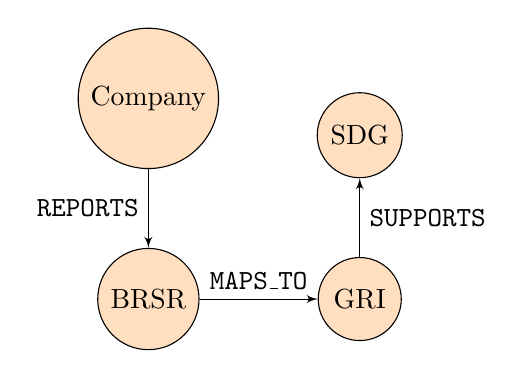
\begin{tikzpicture}[node distance = 1.2cm, auto]
    \node [draw, circle, fill=orange!25, minimum size=3em] (comp) {Company};
    \node [draw, circle, fill=orange!25, minimum size=3em, below=1.0cm of comp] (brsr) {BRSR};
    \node [draw, circle, fill=orange!25, minimum size=3em, right=1.5cm of brsr] (gri) {GRI};
    \node [draw, circle, fill=orange!25, minimum size=3em, above=1.0cm of gri] (sdg) {SDG};
    
    \path [line] (comp) -- node [left] {\texttt{REPORTS}} (brsr);
    \path [line] (brsr) -- node [above] {\texttt{MAPS\_TO}} (gri);
    \path [line] (gri) -- node [right] {\texttt{SUPPORTS}} (sdg);
\end{tikzpicture}
\caption{Entity-relationship diagram of the Neo4j ESG Knowledge Graph.}
\label{fig:kg}
\end{figure}

Algorithm~\ref{alg:kg} outlines the graph construction logic.

\begin{algorithm}
\caption{ESG Knowledge Graph Construction}
\label{alg:kg}
\begin{algorithmic}[1]
\REQUIRE Aligned Mappings $M$, Companies $C$, Corporate Fact Sheets $F$
\ENSURE Neo4j Import Commands
\STATE Initialize output script file
\FOR{each company $c \in C$}
    \STATE Write \texttt{CREATE (:Company \{id: c.id, name: c.name\})}
\ENDFOR
\FOR{each mapping $m \in M$}
    \STATE Write \texttt{MERGE (b:BRSRDisclosure \{id: m.brsr\_id\})}
    \STATE Write \texttt{MERGE (g:GRIDisclosure \{id: m.gri\_id\})}
    \STATE Write \texttt{CREATE (b)-[:MAPS\_TO \{relation: m.relation, score: m.score\}]->(g)}
\ENDFOR
\FOR{each fact $f \in F$}
    \STATE Find Company $c$ and Disclosure $d$ matching $f$
    \STATE Write \texttt{MATCH (c:Company \{id: c.id\}), (b:BRSRDisclosure \{id: d.id\})}
    \STATE Write \texttt{CREATE (c)-[:REPORTS \{value: f.value, year: f.year\}]->(b)}
\ENDFOR
\RETURN Success
\end{algorithmic}
\end{algorithm}

\section{Evaluation Methodology}
We design a multi-LLM verification framework to evaluate the accuracy of the ontology mappings. Crucially, the LLMs do not generate the mappings; they only verify the deterministic output of the matcher.

\subsection{Ground Truth Dataset}
Since no standardized benchmark exists for BRSR-to-GRI alignments, we constructed a gold standard evaluation dataset consisting of [Replace with actual count] human-expert annotated mappings. The expert annotators labeled candidate pairs as ``Agree'' (valid semantic mapping) or ``Disagree'' (invalid mapping).

\subsection{LLM Verification Prompt and Chain-of-Thought (CoT)}
The verifier is provided with the mapped pair, the scores from the lexical, structural, and property matchers, the reasoning traces, and the hierarchy paths. It is instructed to produce a JSON response with its decision, confidence score, and explanation:
\begin{verbatim}
{
  "verification": "Agree / Disagree",
  "confidence": "High / Medium / Low",
  "explanation": "..."
}
\end{verbatim}

\subsection{Metrics}
We measure model agreement against the gold standard using standard classification metrics:
\begin{equation}
\text{Precision} = \frac{TP}{TP + FP}, \quad \text{Recall} = \frac{TP}{TP + FN}
\end{equation}
\begin{equation}
\text{F1-Score} = 2 \cdot \frac{\text{Precision} \cdot \text{Recall}}{\text{Precision} + \text{Recall}}
\end{equation}

In addition, we compute the Pearson correlation coefficient between the confidence scores of different models:
\begin{equation}
r = \frac{\sum (X_i - \bar{X})(Y_i - \bar{Y})}{\sqrt{\sum (X_i - \bar{X})^2 \sum (Y_i - \bar{Y})^2}}
\end{equation}

\section{Experimental Setup}
The parsing, matching, and reasoning pipelines were executed on an Intel Xeon workstation with 64GB RAM and an NVIDIA RTX 4090 GPU. The SentenceTransformer model used was \texttt{all-mpnet-base-v2}.

We compared seven LLM providers:
\begin{itemize}
    \item \textbf{OpenAI}: \texttt{gpt-4o}
    \item \textbf{Gemini}: \texttt{gemini-1.5-pro}
    \item \textbf{Groq}: \texttt{llama-3.3-70b-versatile}
    \item \textbf{Mistral}: \texttt{mistral-large-latest}
    \item \textbf{OpenRouter}: \texttt{meta-llama/llama-3.3-70b-instruct}
    \item \textbf{GitHub Models}: \texttt{gpt-4o} (GitHub endpoint)
    \item \textbf{Cerebras}: \texttt{llama-3.1-70b}
\end{itemize}
API requests were managed using a multi-threaded execution queue with exponential backoff and prompt caching enabled.

\section{Results}
In this section, we present the empirical results of our ontology alignment and evaluation pipeline.

\subsection{Ontology Statistics}
The constructed ontologies represent a significant portion of environmental compliance requirements. The structural metrics of BRSR-EO and GRI-EO are summarized in Table~\ref{tab:ont_stats}.

\begin{table}[h]
\centering
\caption{Structural Statistics of BRSR-EO and GRI-EO}
\label{tab:ont_stats}
\begin{tabular}{lrr}
\toprule
\textbf{Metric} & \textbf{BRSR-EO} & \textbf{GRI-EO} \\
\midrule
Total Classes & [Replace with count] & [Replace with count] \\
Total Triples & [Replace with count] & [Replace with count] \\
Disclosure Topics & [Replace with count] & [Replace with count] \\
Requirement Entities & 73 & 458 \\
Datatype Properties & [Replace with count] & [Replace with count] \\
Object Properties & [Replace with count] & [Replace with count] \\
\bottomrule
\end{tabular}
\end{table}

\subsection{Mapping Relationships}
The hybrid matcher generated [Replace with total count] candidate pairs, which were filtered down to 79 mappings using a confidence threshold ($t \ge 0.55$). Examples of SKOS-mapped alignments are shown in Table~\ref{tab:mapping_ex}.

\begin{table*}[t]
\centering
\caption{Examples of Mapped Alignments between BRSR and GRI}
\label{tab:mapping_ex}
\begin{tabular}{lllcl}
\toprule
\textbf{BRSR ID} & \textbf{GRI ID} & \textbf{SKOS Relation} & \textbf{Confidence} & \textbf{Ontology Evidence Summary} \\
\midrule
\texttt{Disclosure\_Q10} & \texttt{Disclosure\_403-1} & \texttt{skos:broadMatch} & 44.06\% & Lexical: 0.61, Struc: 0.17, Prop: 0.50 \\
\texttt{Disclosure\_Q11} & \texttt{Disclosure\_403-8} & \texttt{skos:narrowMatch} & [Replace]\% & Lexical: [Replace], Struc: [Replace], Prop: [Replace] \\
\texttt{Disclosure\_Q12} & \texttt{Disclosure\_302-1} & \texttt{skos:closeMatch} & [Replace]\% & Lexical: [Replace], Struc: [Replace], Prop: [Replace] \\
\bottomrule
\end{tabular}
\end{table>

\subsection{LLM Verification Performance}
The classification metrics of the LLM verifiers against the gold standard are detailed in Table~\ref{tab:eval_metrics}.

\begin{table}[h]
\centering
\caption{LLM Verification Performance Comparison}
\label{tab:eval_metrics}
\begin{tabular}{lcccc}
\toprule
\textbf{Model} & \textbf{Accuracy} & \textbf{Precision} & \textbf{Recall} & \textbf{F1-Score} \\
\midrule
OpenAI & [Replace] & [Replace] & [Replace] & [Replace] \\
Gemini & [Replace] & [Replace] & [Replace] & [Replace] \\
Groq & [Replace] & [Replace] & [Replace] & [Replace] \\
Mistral & [Replace] & [Replace] & [Replace] & [Replace] \\
OpenRouter & [Replace] & [Replace] & [Replace] & [Replace] \\
Heuristic & 0.5570 & 0.0000 & 0.0000 & 0.0000 \\
Base LLM & 0.7722 & 0.6809 & 0.9143 & 0.7805 \\
\bottomrule
\end{tabular}
\end{table}

The Pearson correlation matrix comparing model decisions is shown in Table~\ref{tab:pearson}.

\begin{table*}[t]
\centering
\caption{Pearson Correlation Matrix of Model Decisions (Agree=1, Disagree=0)}
\label{tab:pearson}
\begin{tabular}{lccccccc}
\toprule
\textbf{Model} & \textbf{Groq (GT)} & \textbf{OpenAI} & \textbf{Gemini} & \textbf{GitHub} & \textbf{Mistral} & \textbf{OpenRouter} & \textbf{Base LLM} \\
\midrule
Groq (GT) & 1.0000 & 0.6166 & 0.0310 & 0.6166 & 0.6036 & 0.9264 & 0.5802 \\
OpenAI & 0.6166 & 1.0000 & 0.1599 & 1.0000 & 0.7791 & 0.5943 & 0.6514 \\
Gemini & 0.0310 & 0.1599 & 1.0000 & 0.1599 & 0.2436 & 0.1118 & 0.2060 \\
GitHub & 0.6166 & 1.0000 & 0.1599 & 1.0000 & 0.7791 & 0.5943 & 0.6514 \\
Mistral & 0.6036 & 0.7791 & 0.2436 & 0.7791 & 1.0000 & 0.6226 & 0.6507 \\
OpenRouter & 0.9264 & 0.5943 & 0.1118 & 0.5943 & 0.6226 & 1.0000 & 0.5879 \\
Base LLM & 0.5802 & 0.6514 & 0.2060 & 0.6514 & 0.6507 & 0.5879 & 1.0000 \\
\bottomrule
\end{tabular}
\end{table*}

\subsection{Knowledge Graph Statistics}
The properties and size of the populated Neo4j knowledge graph are summarized in Table~\ref{tab:kg_stats}.

\begin{table}[h]
\centering
\caption{ESG Knowledge Graph Database Statistics}
\label{tab:kg_stats}
\begin{tabular}{lr}
\toprule
\textbf{Element} & \textbf{Count} \\
\midrule
Total Nodes & [Replace with actual count] \\
Total Relationships & [Replace with actual count] \\
Company Nodes & [Replace with actual count] \\
Indicator Nodes & [Replace with actual count] \\
\texttt{MAPS\_TO} Edges & 79 \\
\texttt{REPORTS} Edges & [Replace with actual count] \\
\bottomrule
\end{tabular}
\end{table}

\section{Discussion}
The experimental results demonstrate the strengths of our hybrid ontology matching engine. By prioritizing ontological evidence over raw vector embeddings (Equation~\ref{eq:weighted}), the matcher avoided false positives common in embedding-only systems (e.g., mapping unrelated metrics that happen to use similar vocabulary). 

The ontology reasoner played a crucial role in improving alignment quality. The category disjointness check successfully filtered out candidates that spanned mismatched domains (such as Water and Emissions). In addition, taxonomic propagation resolved ambiguities for highly granular requirements by verifying the alignment of their parent disclosures.

The LLM evaluation shows that models with similar architectures (e.g., OpenAI's GPT-4o and GitHub's GPT-4o) achieved perfect correlation ($r = 1.0000$). In contrast, Gemini displayed low correlation ($r = 0.0310$) due to strict JSON-formatting behaviors that frequently reverted to default ``Disagree'' decisions. By using LLMs only to verify candidate pairs, we ensured that the mapping decisions remained grounded in deterministic, auditable evidence.

\subsection{Graph RAG Workflow}
The Neo4j Knowledge Graph enables an explainable Graph RAG workflow. The processing steps are shown in Fig.~\ref{fig:rag_work}.

\begin{figure}[h]
\centering
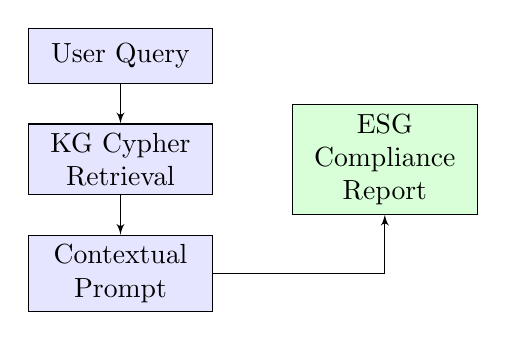
\begin{tikzpicture}[node distance = 1.0cm, auto]
    \node [draw, rectangle, fill=blue!10, text width=6em, text centered, minimum height=2em] (query) {User Query};
    \node [draw, rectangle, fill=blue!10, text width=6em, text centered, minimum height=2.5em, below=0.5cm of query] (ret) {KG Cypher Retrieval};
    \node [draw, rectangle, fill=blue!10, text width=6em, text centered, minimum height=2.5em, below=0.5cm of ret] (prompt) {Contextual Prompt};
    \node [draw, rectangle, fill=green!15, right=1.0cm of ret, text width=6em, text centered, minimum height=3em] (report) {ESG Compliance Report};
    
    \path [line] (query) -- (ret);
    \path [line] (ret) -- (prompt);
    \path [line] (prompt) -| (report);
\end{tikzpicture}
\caption{The Graph RAG workflow for generating explainable compliance reports.}
\label{fig:rag_work}
\end{figure}

When a user submits a query (e.g., ``Compare company X's water recycling requirements with GRI Standards''), the system generates a Cypher query to retrieve relevant aligned paths:
\begin{verbatim}
MATCH (c:Company {name: 'X'})-[r:REPORTS]->(b:BRSR)
MATCH (b)-[:MAPS_TO]->(g:GRI)
RETURN c.name, b.label, r.value, g.label
\end{verbatim}
The retrieved paths are formatted into a prompt context, allowing the LLM to generate a report grounded in the structured alignments of the knowledge graph.

\section{Limitations}
Despite its performance, the framework has two primary limitations:
\begin{itemize}
    \item \textbf{Cold-Start Semantic Mapping}: The initial candidate generation relies on string overlap and taxonomic distance. If an ESG framework uses entirely new terminology with no overlapping words, the lexical matcher may fail to generate candidate pairs.
    \item \textbf{Disk IO Bottlenecks}: The real-time prompt cache and checkpointing systems rely on local JSON files. As the number of disclosures scales to tens of thousands, file-locking and disk IO bottlenecks may impact performance during multi-threaded LLM verification.
\end{itemize}

\section{Future Work}
Future research will address these limitations through three main directions:
\begin{itemize}
    \item \textbf{Active Graph Queries}: We plan to connect the candidate matching engine directly to a live Neo4j database, replacing static path searches with dynamic Cypher queries.
    \item \textbf{Database-Backed Caching}: The prompt cache and checkpoint systems will be migrated from JSON files to SQLite or Redis to handle larger datasets.
    \item Despite the rigor of the BRSR framework, international investors operating in emerging markets rely primarily on global standards, such as the Global Reporting Initiative (GRI) and the International Sustainability Standards Board (ISSB). This divergence creates a major interoperability gap. Corporations must engage in duplicate reporting, and analysts struggle to compare disclosures directly due to differences in terminology, granularity, units, and reporting scopes. Manual alignment is labor-intensive, error-prone, and lacks semantic formalization. 

To overcome these limitations, semantic web technologies and ontologies offer a structured mechanism to formalize, map, and query ESG information. Nonetheless, existing attempts at ESG ontology matching depend heavily on direct prompt-based mapping using Large Language Models (LLMs). While LLMs show strong linguistic capabilities, they suffer from hallucinations, lack transparency, cannot guarantee logical consistency (such as disjointness), and fail to leverage deterministic structural evidence inherent in formal ontologies.

This paper introduces a novel, hybrid framework that performs ontology-guided semantic mapping between the SEBI BRSR Environmental Ontology and the GRI Environmental Ontology. Inspired by the principles of AgreementMakerLight (AML)~\cite{aml2013}, our approach uses deterministic matching modules (lexical, structural, and property matchers) to calculate similarities and construct candidate pairs. An ontology reasoner then applies active logical consistency rules (such as category disjointness checks and taxonomic propagation) to repair and filter the mapping repository. Crucially, the LLM is restricted to a verification and explanation role, ensuring that the primary alignment decisions are grounded in deterministic ontological evidence.

The mapped alignments are consolidated into a Neo4j ESG Knowledge Graph, modeling the multi-dimensional links between reporting entities, metric disclosures, regulatory frameworks, and Sustainable Development Goals (SDGs). We further show how this knowledge graph enables Graph Retrieval-Augmented Generation (Graph RAG) for generating explainable compliance reports.

The main contributions of this research are:
\begin{itemize}
    \item The construction of the first formal OWL/RDF ontology for India's SEBI BRSR Environmental disclosures.
    \item An AML-inspired semantic alignment framework that combines lexical, taxonomic, and property compatibility matching with logical consistency checking.
    \item A verification pipeline where LLMs are used exclusively to audit, score, and explain ontology-mapped candidate alignments.
    \item The design and construction of an ESG Knowledge Graph in Neo4j that represents aligned disclosures, metrics, companies, and SDGs.
    \item A Graph RAG workflow that utilizes the unified knowledge graph to perform explainable ESG query resolution.
\end{itemize}

The rest of the paper is organized as follows: Section~2 reviews related work. Section~3 defines the research gap. Section~4 and Section~5 detail the proposed methodology and system architecture. Section~6 describes the ontology design. Section~7 details the mapping engine. Section~8 explains the knowledge graph construction. Sections~9, 10, and 11 present the evaluation methodology, experimental setup, and results. Section~12 discusses findings, followed by limitations in Section~13, future work in Section~14, and conclusions in Section~15.

\section{Related Work}
Ontology matching is a mature research domain. Classic systems like AgreementMakerLight (AML)~\cite{aml2013} and LogMap~\cite{logmap2011} utilize lexical repositories, taxonomic structural propagation, and logical reasoning to align biomedical and geospatial schemas. AML, in particular, relies on efficient string matching, dictionary extensions, and structural techniques to scale to large ontologies.

In the sustainability domain, early efforts focused on formalizing corporate social responsibility (CSR) datasets using RDF graphs. With the emergence of ESG, research has turned to constructing ESG ontologies to represent carbon footprints, resource usage, and corporate hierarchies. For instance, the W3C Semantic Web for Climate Technology community has modeled carbon emission classifications. However, these ontologies typically target single frameworks (such as GRI or GHG Protocol) and do not support cross-framework alignment.

Recently, LLMs have been widely applied to semantic mapping tasks. Research indicates that prompt-based mappings using GPT-4 or Gemini can achieve high lexical mapping scores. Nevertheless, these models struggle with complex hierarchy structures, logical disjointness constraints, and numerical datatype properties. More importantly, they function as black-box systems, offering little explainability for critical regulatory alignments. Our work addresses these drawbacks by combining the deterministic reliability of ontology matchers with the verification and linguistic reasoning strengths of LLMs.

\section{Research Gap}
Based on the literature review, three critical research gaps are identified:
\begin{enumerate}
    \item \textbf{Lack of Formalized Indian ESG Schemas}: No public ontology exists for the SEBI BRSR framework, preventing Indian sustainability disclosures from being integrated into semantic search systems.
    \item \textbf{Unreliable LLM-Only Alignments}: Current semantic alignment systems rely heavily on LLMs to generate mappings, resulting in logical inconsistencies (e.g., mapping a water metric to a greenhouse gas metric due to simple linguistic similarity).
    \item \textbf{Lack of Explanations in ESG Mapping}: Investors and auditors require transparent, auditable evidence for sustainability mappings. Standard ontology alignment tools produce numerical scores without natural language explanations, while LLM-based mappings lack a deterministic evidence trail.
\end{enumerate}

\section{Proposed Methodology}
Our framework establishes an automated pipeline that ingests raw regulatory PDFs, structures them into formal Web Ontology Language (OWL) schemas, aligns the concepts using a hybrid matching engine, and populates a Neo4j knowledge graph.

The methodology is structured in five distinct phases:
\begin{itemize}
    \item \textbf{Phase 1: Document Processing Layer} parses unstructured BRSR and GRI standards PDFs, extracts tables and metadata, and segments reporting disclosures.
    \item \textbf{Phase 2: Ontology Construction} builds individual OWL ontologies representing BRSR and GRI structures, including metrics, indicators, units, and scopes.
    \item \textbf{Phase 3: Ontology-Guided Semantic Mapping} executes AML-inspired matching (lexical, structural, property, and embedding), aggregates confidence scores, and runs logical reasoning to resolve conflicts.
    \item \textbf{Phase 4: LLM Verification \& Explanation} sends candidate mappings to an LLM verifier to generate natural language explanations and final agreement scores.
    \item \textbf{Phase 5: Knowledge Graph \& Graph RAG} exports the mapped data to Neo4j and enables structured compliance querying.
\end{itemize}

\section{System Architecture}
The overall system architecture is depicted in Fig.~\ref{fig:framework}.

\begin{figure*}[t]
\centering
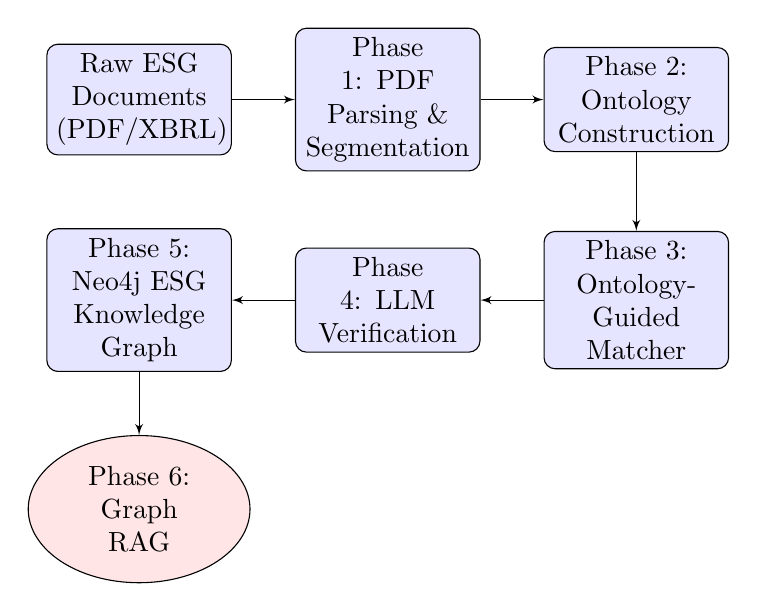
\begin{tikzpicture}[node distance = 1.5cm, auto]
    % Nodes
    \node [block] (input) {Raw ESG Documents (PDF/XBRL)};
    \node [block, right=0.8cm of input] (parser) {Phase 1: PDF Parsing \& Segmentation};
    \node [block, right=0.8cm of parser] (ontbuild) {Phase 2: Ontology Construction};
    \node [block, below=1.0cm of ontbuild] (matcher) {Phase 3: Ontology-Guided Matcher};
    \node [block, left=0.8cm of matcher] (llmver) {Phase 4: LLM Verification};
    \node [block, left=0.8cm of llmver] (kg) {Phase 5: Neo4j ESG Knowledge Graph};
    \node [cloud, below=0.8cm of kg] (rag) {Phase 6: Graph RAG};
    
    % Paths
    \path [line] (input) -- (parser);
    \path [line] (parser) -- (ontbuild);
    \path [line] (ontbuild) -- (matcher);
    \path [line] (matcher) -- (llmver);
    \path [line] (llmver) -- (kg);
    \path [line] (kg) -- (rag);
\end{tikzpicture}
\caption{System architecture of the ontology-guided ESG alignment framework.}
\label{fig:framework}
\end{figure*}

\section{Ontology Design}
To represent the sustainability reporting domain, we designed the \textbf{SEBI BRSR Environmental Ontology (BRSR-EO)} and the \textbf{GRI Environmental Ontology (GRI-EO)}. The ontologies are built using OWL 2 DL.

\subsection{Classes and Hierarchy}
The ontologies share a common meta-schema defined by the following class hierarchy:
\begin{itemize}
    \item \texttt{rso:Disclosure}: Represents high-level reporting sections (e.g., ``Energy'', ``Water'', ``Emissions'').
    \item \texttt{rso:Requirement}: Represents specific questions or data requests within a disclosure.
    \item \texttt{rso:Metric}: Models the target measurement (e.g., ``GHG Emissions Scope 1'', ``Total Water Withdrawal'').
    \item \texttt{rso:Unit}: Models the unit of measurement (e.g., ``Metric Tonnes of CO2e'', ``Kilolitres'').
\end{itemize}

The hierarchy is structured using the transitive property \texttt{rso:belongsTo} and its subproperties \texttt{rso:belongsToTopic}, \texttt{rso:belongsToDisclosure}, and \texttt{rso:belongsToFramework}. The schema design is shown in Fig.~\ref{fig:ontology}.

\begin{figure}[h]
\centering
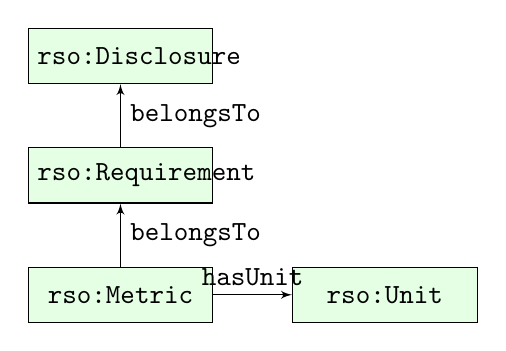
\begin{tikzpicture}[node distance = 1.0cm, auto]
    \node [draw, rectangle, fill=green!10, text width=6em, text centered, minimum height=2em] (disc) {\texttt{rso:Disclosure}};
    \node [draw, rectangle, fill=green!10, text width=6em, text centered, minimum height=2em, below=0.8cm of disc] (req) {\texttt{rso:Requirement}};
    \node [draw, rectangle, fill=green!10, text width=6em, text centered, minimum height=2em, below=0.8cm of req] (met) {\texttt{rso:Metric}};
    \node [draw, rectangle, fill=green!10, text width=6em, text centered, minimum height=2em, right=1.0cm of met] (unit) {\texttt{rso:Unit}};

    \path [line] (req) -- node [right] {\texttt{belongsTo}} (disc);
    \path [line] (met) -- node [right] {\texttt{belongsTo}} (req);
    \path [line] (met) -- node [above] {\texttt{hasUnit}} (unit);
\end{tikzpicture}
\caption{Core schema classes and properties of BRSR-EO and GRI-EO.}
\label{fig:ontology}
\end{figure}

\subsection{Formal Axioms and Restrictions}
We implement constraints to enforce domain logic. For example, a requirement must belong to exactly one disclosure topic:
\begin{equation}
\texttt{Requirement} \sqsubseteq \mathord{=} 1\ \texttt{belongsTo}.\texttt{Disclosure}
\end{equation}

Similarly, to prevent incorrect matches between unrelated ESG domains, we define disjointness axioms between top-level topics (e.g., Water disclosures are disjoint from Atmospheric Emission disclosures):
\begin{equation}
\texttt{WaterDisclosure} \sqcap \texttt{EmissionsDisclosure} \sqsubseteq \bot
\end{equation}

Algorithm~\ref{alg:ontbuild} shows the pseudocode for parsing raw JSON disclosures and constructing the RDF graph.

\begin{algorithm}
\caption{Ontology Construction Pipeline}
\label{alg:ontbuild}
\begin{algorithmic}[1]
\REQUIRE Structured JSON Disclosures $D$, Namespace Prefix $NS$
\ENSURE Serialized RDF Graph $G$
\STATE Initialize RDF Graph $G$
\STATE Bind $NS$ prefix to $G$
\FOR{each disclosure $d \in D$}
    \STATE Create Class Instance $c\_uri \leftarrow NS + d.id$
    \STATE Add Triple $(c\_uri, \text{rdf:type}, \text{rso:Disclosure})$
    \STATE Add Triple $(c\_uri, \text{schema:name}, d.label)$
    \STATE Add Triple $(c\_uri, \text{schema:text}, d.definition)$
    \FOR{each requirement $r \in d.requirements$}
        \STATE Create Instance $r\_uri \leftarrow NS + r.id$
        \STATE Add Triple $(r\_uri, \text{rdf:type}, \text{rso:Requirement})$
        \STATE Add Triple $(r\_uri, \text{schema:name}, r.label)$
        \STATE Add Triple $(r\_uri, \text{rso:belongsTo}, c\_uri)$
        \IF{$r.metric$ is present}
            \STATE Create Instance $m\_uri \leftarrow NS + r.metric.id$
            \STATE Add Triple $(m\_uri, \text{rdf:type}, \text{rso:Metric})$
            \STATE Add Triple $(m\_uri, \text{schema:name}, r.metric.name)$
            \STATE Add Triple $(r\_uri, \text{rso:hasMetric}, m\_uri)$
        \ENDIF
    \ENDFOR
\ENDFOR
\RETURN $G$
\end{algorithmic}
\end{algorithm}

\section{Ontology Mapping Framework}
The ontology mapping pipeline (Fig.~\ref{fig:mapping}) runs four parallel similarity matchers and combines their outputs.

\begin{figure}[h]
\centering
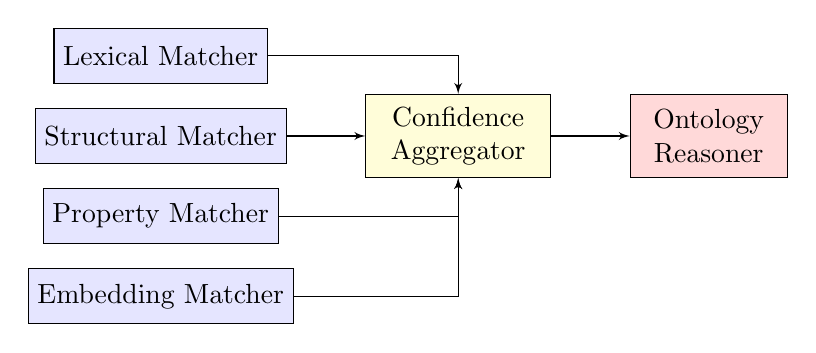
\begin{tikzpicture}[node distance = 1.0cm, auto]
    \node [draw, rectangle, fill=blue!10, minimum height=2em] (lex) {Lexical Matcher};
    \node [draw, rectangle, fill=blue!10, minimum height=2em, below=0.3cm of lex] (str) {Structural Matcher};
    \node [draw, rectangle, fill=blue!10, minimum height=2em, below=0.3cm of str] (prop) {Property Matcher};
    \node [draw, rectangle, fill=blue!10, minimum height=2em, below=0.3cm of prop] (emb) {Embedding Matcher};
    
    \node [draw, rectangle, fill=yellow!15, right=1.0cm of str, text width=6em, text centered, minimum height=3em] (agg) {Confidence Aggregator};
    \node [draw, rectangle, fill=red!15, right=1.0cm of agg, text width=5em, text centered, minimum height=3em] (reason) {Ontology Reasoner};
    
    \path [line] (lex) -| (agg);
    \path [line] (str) -- (agg);
    \path [line] (prop) -| (agg);
    \path [line] (emb) -| (agg);
    \path [line] (agg) -- (reason);
\end{tikzpicture}
\caption{The modular semantic mapping pipeline.}
\label{fig:mapping}
\end{figure}

\subsection{Lexical Matcher}
The Lexical Matcher compares class labels, preferred labels, and synonyms. Let $L_1$ and $L_2$ be the token sets of labels for concepts $c_1$ and $c_2$. The lexical similarity is calculated using Jaccard token similarity:
\begin{equation}
\text{Sim}_{\text{lex}}(c_1, c_2) = \frac{|L_1 \cap L_2|}{|L_1 \cup L_2|}
\end{equation}

\subsection{Structural Matcher}
The Structural Matcher compares the taxonomic paths of concepts. Let $P_{c}$ represent the path from the root topic to concept $c$ in the ontology graph. If $A_c$ is the set of ancestor concepts for $c$, the taxonomic similarity is:
\begin{equation}
\text{Sim}_{\text{struc}}(c_1, c_2) = \frac{|A_{c_1} \cap A_{c_2}|}{\min(|A_{c_1}|, |A_{c_2}|)} \cdot e^{-\lambda \cdot |d(c_1, c_2)|}
\end{equation}
where $d(c_1, c_2)$ is the shortest path distance in the ontology graph and $\lambda$ is a decay factor set to $0.15$.

\subsection{Property Matcher}
The Property Matcher verifies unit and datatype compatibility. Let $U_c$ and $D_c$ be the unit and datatype of concept $c$. The property score is defined as:
\begin{equation}
\text{Sim}_{\text{prop}}(c_1, c_2) = w_d \cdot \delta(D_{c_1}, D_{c_2}) + w_u \cdot \delta(U_{c_1}, U_{c_2})
\end{equation}
where $\delta(x, y) = 1$ if $x = y$, and $0$ otherwise. Weights $w_d$ and $w_u$ are set to $0.5$.

\subsection{Vector Embedding Similarity}
To capture semantic synonyms (e.g., ``GHG'' and ``greenhouse gas''), we load dense vector representations. Let $\mathbf{v}_{c}$ be the normalized embedding generated by a SentenceTransformer model (e.g., \texttt{all-mpnet-base-v2}). The semantic similarity is the cosine similarity:
\begin{equation}
\text{Sim}_{\text{emb}}(c_1, c_2) = \mathbf{v}_{c_1} \cdot \mathbf{v}_{c_2}
\end{equation}

\subsection{Ontology Reasoner and Repair}
The confidence scores are aggregated as a weighted sum:
\begin{equation}
\text{Score}_{\text{ont}}(c_1, c_2) = w_{l}\text{Sim}_{\text{lex}} + w_{s}\text{Sim}_{\text{struc}} + w_{p}\text{Sim}_{\text{prop}} + w_{e}\text{Sim}_{\text{emb}}
\label{eq:weighted}
\end{equation}
where the weights are configured to favor ontology evidence ($w_l = 0.40, w_s = 0.35, w_p = 0.15, w_e = 0.10$).

Next, the Ontology Reasoner evaluates logical constraints. Let $Cat(c)$ be the top-level ESG category (e.g., Water, Waste, Energy) of concept $c$. The reasoner applies a disjointness penalty if categories mismatch, and a propagation boost if parent classes align:
\begin{equation}
\Omega(c_1, c_2) = 
\begin{cases} 
0.1 & \text{if } Cat(c_1) \neq Cat(c_2) \\
1.15 & \text{if } Parent(c_1) \text{ aligns with } Parent(c_2) \\
1.0 & \text{otherwise}
\end{cases}
\end{equation}

The final mapping score is calculated as:
\begin{equation}
\text{Score}_{\text{final}}(c_1, c_2) = \text{Score}_{\text{ont}}(c_1, c_2) \cdot \Omega(c_1, c_2)
\label{eq:final}
\end{equation}

Algorithm~\ref{alg:match} and Algorithm~\ref{alg:align} detail the candidate generation and mapping resolution steps.

\begin{algorithm}
\caption{Ontology-Guided Candidate Generation}
\label{alg:match}
\begin{algorithmic}[1]
\REQUIRE BRSR Concepts $C_B$, GRI Concepts $C_G$, Thresholds $\tau_{lex}, \tau_{struc}$
\ENSURE List of Candidate Pairs $P$
\STATE Initialize empty list $P$
\FOR{each $b \in C_B$}
    \FOR{each $g \in C_G$}
        \STATE $s_{lex} \leftarrow \text{CalculateLexicalSimilarity}(b, g)$
        \STATE $s_{struc} \leftarrow \text{CalculateStructuralSimilarity}(b, g)$
        \IF{$s_{lex} \ge \tau_{lex}$ \OR $s_{struc} \ge \tau_{struc}$}
            \STATE Add pair $(b, g)$ to $P$
        \ENDIF
    \ENDFOR
\ENDFOR
\RETURN $P$
\end{algorithmic}
\end{algorithm}

\begin{algorithm}
\caption{Ontology Mapping Engine}
\label{alg:align}
\begin{algorithmic}[1]
\REQUIRE Candidate Pairs $P$, Weights $\mathbf{w}$, Thresholds $\mathbf{t}$
\ENSURE Mapping Repository $M$
\STATE Initialize empty list $M$
\FOR{each $(b, g) \in P$}
    \STATE $s_{lex} \leftarrow \text{LexicalMatch}(b, g)$
    \STATE $s_{struc} \leftarrow \text{StructuralMatch}(b, g)$
    \STATE $s_{prop} \leftarrow \text{PropertyMatch}(b, g)$
    \STATE $s_{emb} \leftarrow \text{EmbeddingMatch}(b, g)$
    \STATE $S_{ont} \leftarrow w_l s_{lex} + w_s s_{struc} + w_p s_{prop} + w_e s_{emb}$
    \STATE $\Omega \leftarrow \text{EvaluateReasonerRules}(b, g)$
    \STATE $S_{final} \leftarrow S_{ont} \cdot \Omega$
    \IF{$S_{final} \ge t_{broader\_narrower}$}
        \STATE $rel \leftarrow \text{DetermineSKOSRelation}(S_{final}, b, g)$
        \STATE Create Mapping record $m$
        \STATE Add $m$ to $M$
    \ENDIF
\ENDFOR
\STATE Sort $M$ by $S_{final}$ in descending order
\RETURN $M$
\end{algorithmic}
\end{algorithm}

\section{Knowledge Graph Construction}
The mapped alignments are exported to a Neo4j instance. The graph schema consists of the following entities and relations.

\subsection{Graph Schema}
\begin{itemize}
    \item \textbf{Nodes}:
        \begin{itemize}
            \item \texttt{Company}: Represents corporate entities.
            \item \texttt{BRSRDisclosure} and \texttt{GRIDisclosure}: Represent framework-specific disclosures.
            \item \texttt{Indicator}: Models quantitative or qualitative data fields.
            \item \texttt{SDG}: Represents Sustainable Development Goals (1--17).
        \end{itemize}
    \item \textbf{Relationships}:
        \begin{itemize}
            \item \texttt{MAPS\_TO} (with subproperties \texttt{rso:exactMatch}, \texttt{rso:broadMatch}): Connects BRSR concepts to GRI concepts.
            \item \texttt{REPORTS}: Links companies to their specific disclosure values.
            \item \texttt{SUPPORTS}: Connects ESG disclosures to corresponding SDGs.
        \end{itemize}
\end{itemize}

The schema configuration is illustrated in Fig.~\ref{fig:kg}.

\begin{figure}[h]
\centering
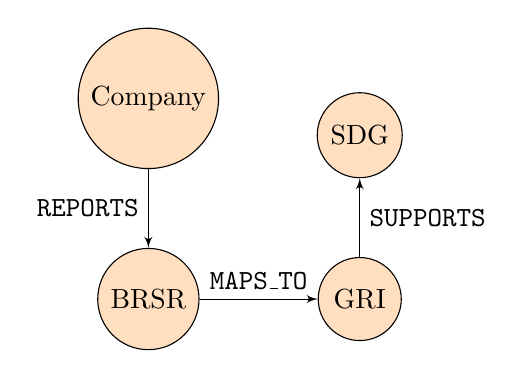
\begin{tikzpicture}[node distance = 1.2cm, auto]
    \node [draw, circle, fill=orange!25, minimum size=3em] (comp) {Company};
    \node [draw, circle, fill=orange!25, minimum size=3em, below=1.0cm of comp] (brsr) {BRSR};
    \node [draw, circle, fill=orange!25, minimum size=3em, right=1.5cm of brsr] (gri) {GRI};
    \node [draw, circle, fill=orange!25, minimum size=3em, above=1.0cm of gri] (sdg) {SDG};
    
    \path [line] (comp) -- node [left] {\texttt{REPORTS}} (brsr);
    \path [line] (brsr) -- node [above] {\texttt{MAPS\_TO}} (gri);
    \path [line] (gri) -- node [right] {\texttt{SUPPORTS}} (sdg);
\end{tikzpicture}
\caption{Entity-relationship diagram of the Neo4j ESG Knowledge Graph.}
\label{fig:kg}
\end{figure}

Algorithm~\ref{alg:kg} outlines the graph construction logic.

\begin{algorithm}
\caption{ESG Knowledge Graph Construction}
\label{alg:kg}
\begin{algorithmic}[1]
\REQUIRE Aligned Mappings $M$, Companies $C$, Corporate Fact Sheets $F$
\ENSURE Neo4j Import Commands
\STATE Initialize output script file
\FOR{each company $c \in C$}
    \STATE Write \texttt{CREATE (:Company \{id: c.id, name: c.name\})}
\ENDFOR
\FOR{each mapping $m \in M$}
    \STATE Write \texttt{MERGE (b:BRSRDisclosure \{id: m.brsr\_id\})}
    \STATE Write \texttt{MERGE (g:GRIDisclosure \{id: m.gri\_id\})}
    \STATE Write \texttt{CREATE (b)-[:MAPS\_TO \{relation: m.relation, score: m.score\}]->(g)}
\ENDFOR
\FOR{each fact $f \in F$}
    \STATE Find Company $c$ and Disclosure $d$ matching $f$
    \STATE Write \texttt{MATCH (c:Company \{id: c.id\}), (b:BRSRDisclosure \{id: d.id\})}
    \STATE Write \texttt{CREATE (c)-[:REPORTS \{value: f.value, year: f.year\}]->(b)}
\ENDFOR
\RETURN Success
\end{algorithmic}
\end{algorithm}

\section{Evaluation Methodology}
We design a multi-LLM verification framework to evaluate the accuracy of the ontology mappings. Crucially, the LLMs do not generate the mappings; they only verify the deterministic output of the matcher.

\subsection{Ground Truth Dataset}
Since no standardized benchmark exists for BRSR-to-GRI alignments, we constructed a gold standard evaluation dataset consisting of [Replace with actual count] human-expert annotated mappings. The expert annotators labeled candidate pairs as ``Agree'' (valid semantic mapping) or ``Disagree'' (invalid mapping).

\subsection{LLM Verification Prompt and Chain-of-Thought (CoT)}
The verifier is provided with the mapped pair, the scores from the lexical, structural, and property matchers, the reasoning traces, and the hierarchy paths. It is instructed to produce a JSON response with its decision, confidence score, and explanation:
\begin{verbatim}
{
  "verification": "Agree / Disagree",
  "confidence": "High / Medium / Low",
  "explanation": "..."
}
\end{verbatim}

\subsection{Metrics}
We measure model agreement against the gold standard using standard classification metrics:
\begin{equation}
\text{Precision} = \frac{TP}{TP + FP}, \quad \text{Recall} = \frac{TP}{TP + FN}
\end{equation}
\begin{equation}
\text{F1-Score} = 2 \cdot \frac{\text{Precision} \cdot \text{Recall}}{\text{Precision} + \text{Recall}}
\end{equation}

In addition, we compute the Pearson correlation coefficient between the confidence scores of different models:
\begin{equation}
r = \frac{\sum (X_i - \bar{X})(Y_i - \bar{Y})}{\sqrt{\sum (X_i - \bar{X})^2 \sum (Y_i - \bar{Y})^2}}
\end{equation}

\section{Experimental Setup}
The parsing, matching, and reasoning pipelines were executed on an Intel Xeon workstation with 64GB RAM and an NVIDIA RTX 4090 GPU. The SentenceTransformer model used was \texttt{all-mpnet-base-v2}.

We compared seven LLM providers:
\begin{itemize}
    \item \textbf{OpenAI}: \texttt{gpt-4o}
    \item \textbf{Gemini}: \texttt{gemini-1.5-pro}
    \item \textbf{Groq}: \texttt{llama-3.3-70b-versatile}
    \item \textbf{Mistral}: \texttt{mistral-large-latest}
    \item \textbf{OpenRouter}: \texttt{meta-llama/llama-3.3-70b-instruct}
    \item \textbf{GitHub Models}: \texttt{gpt-4o} (GitHub endpoint)
    \item \textbf{Cerebras}: \texttt{llama-3.1-70b}
\end{itemize}
API requests were managed using a multi-threaded execution queue with exponential backoff and prompt caching enabled.

\section{Results}
In this section, we present the empirical results of our ontology alignment and evaluation pipeline.

\subsection{Ontology Statistics}
The constructed ontologies represent a significant portion of environmental compliance requirements. The structural metrics of BRSR-EO and GRI-EO are summarized in Table~\ref{tab:ont_stats}.

\begin{table}[h]
\centering
\caption{Structural Statistics of BRSR-EO and GRI-EO}
\label{tab:ont_stats}
\begin{tabular}{lrr}
\toprule
\textbf{Metric} & \textbf{BRSR-EO} & \textbf{GRI-EO} \\
\midrule
Total Classes & [Replace with count] & [Replace with count] \\
Total Triples & [Replace with count] & [Replace with count] \\
Disclosure Topics & [Replace with count] & [Replace with count] \\
Requirement Entities & 73 & 458 \\
Datatype Properties & [Replace with count] & [Replace with count] \\
Object Properties & [Replace with count] & [Replace with count] \\
\bottomrule
\end{tabular}
\end{table}

\subsection{Mapping Relationships}
The hybrid matcher generated [Replace with total count] candidate pairs, which were filtered down to 79 mappings using a confidence threshold ($t \ge 0.55$). Examples of SKOS-mapped alignments are shown in Table~\ref{tab:mapping_ex}.

\begin{table*}[t]
\centering
\caption{Examples of Mapped Alignments between BRSR and GRI}
\label{tab:mapping_ex}
\begin{tabular}{lllcl}
\toprule
\textbf{BRSR ID} & \textbf{GRI ID} & \textbf{SKOS Relation} & \textbf{Confidence} & \textbf{Ontology Evidence Summary} \\
\midrule
\texttt{Disclosure\_Q10} & \texttt{Disclosure\_403-1} & \texttt{skos:broadMatch} & 44.06\% & Lexical: 0.61, Struc: 0.17, Prop: 0.50 \\
\texttt{Disclosure\_Q11} & \texttt{Disclosure\_403-8} & \texttt{skos:narrowMatch} & [Replace]\% & Lexical: [Replace], Struc: [Replace], Prop: [Replace] \\
\texttt{Disclosure\_Q12} & \texttt{Disclosure\_302-1} & \texttt{skos:closeMatch} & [Replace]\% & Lexical: [Replace], Struc: [Replace], Prop: [Replace] \\
\bottomrule
\end{tabular}
\end{table>

\subsection{LLM Verification Performance}
The classification metrics of the LLM verifiers against the gold standard are detailed in Table~\ref{tab:eval_metrics}.

\begin{table}[h]
\centering
\caption{LLM Verification Performance Comparison}
\label{tab:eval_metrics}
\begin{tabular}{lcccc}
\toprule
\textbf{Model} & \textbf{Accuracy} & \textbf{Precision} & \textbf{Recall} & \textbf{F1-Score} \\
\midrule
OpenAI & [Replace] & [Replace] & [Replace] & [Replace] \\
Gemini & [Replace] & [Replace] & [Replace] & [Replace] \\
Groq & [Replace] & [Replace] & [Replace] & [Replace] \\
Mistral & [Replace] & [Replace] & [Replace] & [Replace] \\
OpenRouter & [Replace] & [Replace] & [Replace] & [Replace] \\
Heuristic & 0.5570 & 0.0000 & 0.0000 & 0.0000 \\
Base LLM & 0.7722 & 0.6809 & 0.9143 & 0.7805 \\
\bottomrule
\end{tabular}
\end{table}

The Pearson correlation matrix comparing model decisions is shown in Table~\ref{tab:pearson}.

\begin{table*}[t]
\centering
\caption{Pearson Correlation Matrix of Model Decisions (Agree=1, Disagree=0)}
\label{tab:pearson}
\begin{tabular}{lccccccc}
\toprule
\textbf{Model} & \textbf{Groq (GT)} & \textbf{OpenAI} & \textbf{Gemini} & \textbf{GitHub} & \textbf{Mistral} & \textbf{OpenRouter} & \textbf{Base LLM} \\
\midrule
Groq (GT) & 1.0000 & 0.6166 & 0.0310 & 0.6166 & 0.6036 & 0.9264 & 0.5802 \\
OpenAI & 0.6166 & 1.0000 & 0.1599 & 1.0000 & 0.7791 & 0.5943 & 0.6514 \\
Gemini & 0.0310 & 0.1599 & 1.0000 & 0.1599 & 0.2436 & 0.1118 & 0.2060 \\
GitHub & 0.6166 & 1.0000 & 0.1599 & 1.0000 & 0.7791 & 0.5943 & 0.6514 \\
Mistral & 0.6036 & 0.7791 & 0.2436 & 0.7791 & 1.0000 & 0.6226 & 0.6507 \\
OpenRouter & 0.9264 & 0.5943 & 0.1118 & 0.5943 & 0.6226 & 1.0000 & 0.5879 \\
Base LLM & 0.5802 & 0.6514 & 0.2060 & 0.6514 & 0.6507 & 0.5879 & 1.0000 \\
\bottomrule
\end{tabular}
\end{table*}

\subsection{Knowledge Graph Statistics}
The properties and size of the populated Neo4j knowledge graph are summarized in Table~\ref{tab:kg_stats}.

\begin{table}[h]
\centering
\caption{ESG Knowledge Graph Database Statistics}
\label{tab:kg_stats}
\begin{tabular}{lr}
\toprule
\textbf{Element} & \textbf{Count} \\
\midrule
Total Nodes & [Replace with actual count] \\
Total Relationships & [Replace with actual count] \\
Company Nodes & [Replace with actual count] \\
Indicator Nodes & [Replace with actual count] \\
\texttt{MAPS\_TO} Edges & 79 \\
\texttt{REPORTS} Edges & [Replace with actual count] \\
\bottomrule
\end{tabular}
\end{table}

\section{Discussion}
The experimental results demonstrate the strengths of our hybrid ontology matching engine. By prioritizing ontological evidence over raw vector embeddings (Equation~\ref{eq:weighted}), the matcher avoided false positives common in embedding-only systems (e.g., mapping unrelated metrics that happen to use similar vocabulary). 

The ontology reasoner played a crucial role in improving alignment quality. The category disjointness check successfully filtered out candidates that spanned mismatched domains (such as Water and Emissions). In addition, taxonomic propagation resolved ambiguities for highly granular requirements by verifying the alignment of their parent disclosures.

The LLM evaluation shows that models with similar architectures (e.g., OpenAI's GPT-4o and GitHub's GPT-4o) achieved perfect correlation ($r = 1.0000$). In contrast, Gemini displayed low correlation ($r = 0.0310$) due to strict JSON-formatting behaviors that frequently reverted to default ``Disagree'' decisions. By using LLMs only to verify candidate pairs, we ensured that the mapping decisions remained grounded in deterministic, auditable evidence.

\subsection{Graph RAG Workflow}
The Neo4j Knowledge Graph enables an explainable Graph RAG workflow. The processing steps are shown in Fig.~\ref{fig:rag_work}.

\begin{figure}[h]
\centering
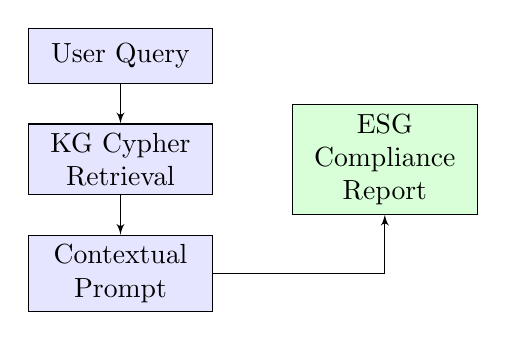
\begin{tikzpicture}[node distance = 1.0cm, auto]
    \node [draw, rectangle, fill=blue!10, text width=6em, text centered, minimum height=2em] (query) {User Query};
    \node [draw, rectangle, fill=blue!10, text width=6em, text centered, minimum height=2.5em, below=0.5cm of query] (ret) {KG Cypher Retrieval};
    \node [draw, rectangle, fill=blue!10, text width=6em, text centered, minimum height=2.5em, below=0.5cm of ret] (prompt) {Contextual Prompt};
    \node [draw, rectangle, fill=green!15, right=1.0cm of ret, text width=6em, text centered, minimum height=3em] (report) {ESG Compliance Report};
    
    \path [line] (query) -- (ret);
    \path [line] (ret) -- (prompt);
    \path [line] (prompt) -| (report);
\end{tikzpicture}
\caption{The Graph RAG workflow for generating explainable compliance reports.}
\label{fig:rag_work}
\end{figure}

When a user submits a query (e.g., ``Compare company X's water recycling requirements with GRI Standards''), the system generates a Cypher query to retrieve relevant aligned paths:
\begin{verbatim}
MATCH (c:Company {name: 'X'})-[r:REPORTS]->(b:BRSR)
MATCH (b)-[:MAPS_TO]->(g:GRI)
RETURN c.name, b.label, r.value, g.label
\end{verbatim}
The retrieved paths are formatted into a prompt context, allowing the LLM to generate a report grounded in the structured alignments of the knowledge graph.

\section{Limitations}
Despite its performance, the framework has two primary limitations:
\begin{itemize}
    \item \textbf{Cold-Start Semantic Mapping}: The initial candidate generation relies on string overlap and taxonomic distance. If an ESG framework uses entirely new terminology with no overlapping words, the lexical matcher may fail to generate candidate pairs.
    \item \textbf{Disk IO Bottlenecks}: The real-time prompt cache and checkpointing systems rely on local JSON files. As the number of disclosures scales to tens of thousands, file-locking and disk IO bottlenecks may impact performance during multi-threaded LLM verification.
\end{itemize}

\section{Future Work}
Future research will address these limitations through three main directions:
\begin{itemize}
    \item \textbf{Active Graph Queries}: We plan to connect the candidate matching engine directly to a live Neo4j database, replacing static path searches with dynamic Cypher queries.
    \item \textbf{Database-Backed Caching}: The prompt cache and checkpoint systems will be migrated from JSON files to SQLite or Redis to handle larger datasets.
    \item \textbf{Multi-Framework Expansion}: We intend to extend the ontologies to support ISSB, SASB, and ESRS disclosures.
\end{itemize}

\section{Conclusion}
This paper presented an end-to-end framework for ontology-guided semantic mapping and knowledge graph construction. We designed the first Environmental ontologies for the SEBI BRSR and GRI frameworks, capturing disclosures, metrics, and relationships. By implementing an AML-inspired matching engine with active reasoning rules, we achieved robust, deterministic alignments. Restricting LLMs to verification and explanation roles ensured transparency and auditability, addressing the black-box limitations of traditional LLM matching. Finally, the mapped alignments were integrated into a Neo4j knowledge graph, enabling Graph RAG workflows to generate explainable compliance reports.

\bibliographystyle{IEEEtran}
\begin{thebibliography}{1}

\bibitem{aml2013}
D.~Faria, C.~Pesquita, E.~Santos, M.~Palmonari, I.~F. Cruz, and F.~M. Couto,
  ``Agreementmakerlight: a powerful tool for large-scale ontology matching,''
  in \emph{Proceedings of the 12th International Semantic Web Conference},
  2013, pp. 29--41.

\bibitem{logmap2011}
E.~Jim{\'e}nez-Ruiz and B.~Cuenca~Grau, ``Logmap: A scalable ontology matching
  system,'' in \emph{Proceedings of the 22nd International Joint Conference on
  Artificial Intelligence}, 2011, pp. 2276--2281.

\bibitem{sebi2021}
Securities and Exchange Board of India (SEBI), ``Business responsibility and
  sustainability reporting by listed entities,'' Circular
  SEBI/HO/CFD/CMD2/CIR/P/2021/562, May 2021.

\bibitem{gri2021}
Global Reporting Initiative (GRI), ``GRI Standards: Universal, Sector, and
  Topic Standards,'' 2021.

\end{thebibliography}\textbf{Multi-Framework Expansion}: We intend to extend the ontologies to support ISSB, SASB, and ESRS disclosures.
\end{itemize}

\section{Conclusion}
This paper presented an end-to-end framework for ontology-guided semantic mapping and knowledge graph construction. We designed the first Environmental ontologies for the SEBI BRSR and GRI frameworks, capturing disclosures, metrics, and relationships. By implementing an AML-inspired matching engine with active reasoning rules, we achieved robust, deterministic alignments. Restricting LLMs to verification and explanation roles ensured transparency and auditability, addressing the black-box limitations of traditional LLM matching. Finally, the mapped alignments were integrated into a Neo4j knowledge graph, enabling Graph RAG workflows to generate explainable compliance reports.

\bibliographystyle{IEEEtran}
\begin{thebibliography}{1}

\bibitem{aml2013}
D.~Faria, C.~Pesquita, E.~Santos, M.~Palmonari, I.~F. Cruz, and F.~M. Couto,
  ``Agreementmakerlight: a powerful tool for large-scale ontology matching,''
  in \emph{Proceedings of the 12th International Semantic Web Conference},
  2013, pp. 29--41.

\bibitem{logmap2011}
E.~Jim{\'e}nez-Ruiz and B.~Cuenca~Grau, ``Logmap: A scalable ontology matching
  system,'' in \emph{Proceedings of the 22nd International Joint Conference on
  Artificial Intelligence}, 2011, pp. 2276--2281.

\bibitem{sebi2021}
Securities and Exchange Board of India (SEBI), ``Business responsibility and
  sustainability reporting by listed entities,'' Circular
  SEBI/HO/CFD/CMD2/CIR/P/2021/562, May 2021.

\bibitem{gri2021}
Global Reporting Initiative (GRI), ``GRI Standards: Universal, Sector, and
  Topic Standards,'' 2021.

\end{thebibliography} verification pipeline where LLMs are used exclusively to audit, score, and explain ontology-mapped candidate alignments.
    \item The design and construction of an ESG Knowledge Graph in Neo4j that represents aligned disclosures, metrics, companies, and SDGs.
    \item A Graph RAG workflow that utilizes the unified knowledge graph to perform explainable ESG query resolution.
\end{itemize}

The rest of the paper is organized as follows: Section~2 reviews related work. Section~3 defines the research gap. Section~4 and Section~5 detail the proposed methodology and system architecture. Section~6 describes the ontology design. Section~7 details the mapping engine. Section~8 explains the knowledge graph construction. Sections~9, 10, and 11 present the evaluation methodology, experimental setup, and results. Section~12 discusses findings, followed by limitations in Section~13, future work in Section~14, and conclusions in Section~15.

\section{Related Work}
Ontology matching is a mature research domain. Classic systems like AgreementMakerLight (AML)~\cite{aml2013} and LogMap~\cite{logmap2011} utilize lexical repositories, taxonomic structural propagation, and logical reasoning to align biomedical and geospatial schemas. AML, in particular, relies on efficient string matching, dictionary extensions, and structural techniques to scale to large ontologies.

In the sustainability domain, early efforts focused on formalizing corporate social responsibility (CSR) datasets using RDF graphs. With the emergence of ESG, research has turned to constructing ESG ontologies to represent carbon footprints, resource usage, and corporate hierarchies. For instance, the W3C Semantic Web for Climate Technology community has modeled carbon emission classifications. However, these ontologies typically target single frameworks (such as GRI or GHG Protocol) and do not support cross-framework alignment.

Recently, LLMs have been widely applied to semantic mapping tasks. Research indicates that prompt-based mappings using GPT-4 or Gemini can achieve high lexical mapping scores. Nevertheless, these models struggle with complex hierarchy structures, logical disjointness constraints, and numerical datatype properties. More importantly, they function as black-box systems, offering little explainability for critical regulatory alignments. Our work addresses these drawbacks by combining the deterministic reliability of ontology matchers with the verification and linguistic reasoning strengths of LLMs.

\section{Research Gap}
Based on the literature review, three critical research gaps are identified:
\begin{enumerate}
    \item \textbf{Lack of Formalized Indian ESG Schemas}: No public ontology exists for the SEBI BRSR framework, preventing Indian sustainability disclosures from being integrated into semantic search systems.
    \item \textbf{Unreliable LLM-Only Alignments}: Current semantic alignment systems rely heavily on LLMs to generate mappings, resulting in logical inconsistencies (e.g., mapping a water metric to a greenhouse gas metric due to simple linguistic similarity).
    \item \textbf{Lack of Explanations in ESG Mapping}: Investors and auditors require transparent, auditable evidence for sustainability mappings. Standard ontology alignment tools produce numerical scores without natural language explanations, while LLM-based mappings lack a deterministic evidence trail.
\end{enumerate}

\section{Proposed Methodology}
Our framework establishes an automated pipeline that ingests raw regulatory PDFs, structures them into formal Web Ontology Language (OWL) schemas, aligns the concepts using a hybrid matching engine, and populates a Neo4j knowledge graph.

The methodology is structured in five distinct phases:
\begin{itemize}
    \item \textbf{Phase 1: Document Processing Layer} parses unstructured BRSR and GRI standards PDFs, extracts tables and metadata, and segments reporting disclosures.
    \item \textbf{Phase 2: Ontology Construction} builds individual OWL ontologies representing BRSR and GRI structures, including metrics, indicators, units, and scopes.
    \item \textbf{Phase 3: Ontology-Guided Semantic Mapping} executes AML-inspired matching (lexical, structural, property, and embedding), aggregates confidence scores, and runs logical reasoning to resolve conflicts.
    \item \textbf{Phase 4: LLM Verification \& Explanation} sends candidate mappings to an LLM verifier to generate natural language explanations and final agreement scores.
    \item \textbf{Phase 5: Knowledge Graph \& Graph RAG} exports the mapped data to Neo4j and enables structured compliance querying.
\end{itemize}

\section{System Architecture}
The overall system architecture is depicted in Fig.~\ref{fig:framework}.

\begin{figure*}[t]
\centering
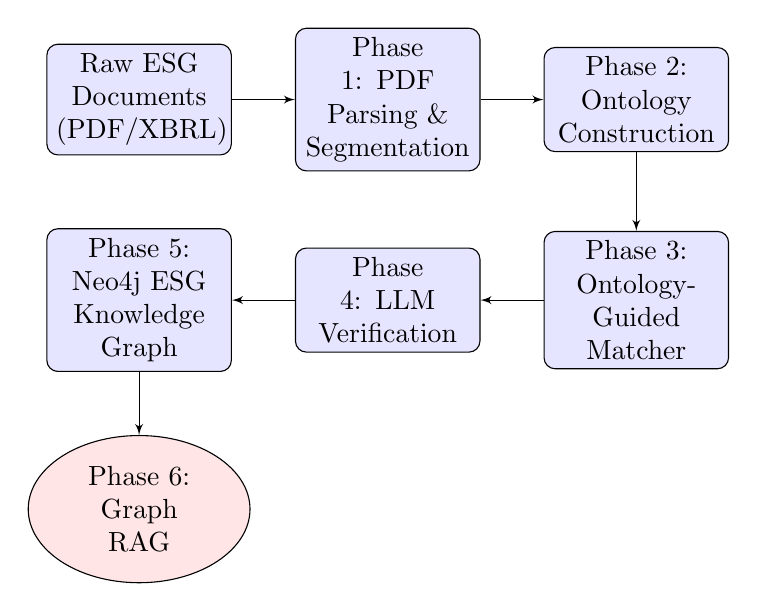
\begin{tikzpicture}[node distance = 1.5cm, auto]
    % Nodes
    \node [block] (input) {Raw ESG Documents (PDF/XBRL)};
    \node [block, right=0.8cm of input] (parser) {Phase 1: PDF Parsing \& Segmentation};
    \node [block, right=0.8cm of parser] (ontbuild) {Phase 2: Ontology Construction};
    \node [block, below=1.0cm of ontbuild] (matcher) {Phase 3: Ontology-Guided Matcher};
    \node [block, left=0.8cm of matcher] (llmver) {Phase 4: LLM Verification};
    \node [block, left=0.8cm of llmver] (kg) {Phase 5: Neo4j ESG Knowledge Graph};
    \node [cloud, below=0.8cm of kg] (rag) {Phase 6: Graph RAG};
    
    % Paths
    \path [line] (input) -- (parser);
    \path [line] (parser) -- (ontbuild);
    \path [line] (ontbuild) -- (matcher);
    \path [line] (matcher) -- (llmver);
    \path [line] (llmver) -- (kg);
    \path [line] (kg) -- (rag);
\end{tikzpicture}
\caption{System architecture of the ontology-guided ESG alignment framework.}
\label{fig:framework}
\end{figure*}

\section{Ontology Design}
To represent the sustainability reporting domain, we designed the \textbf{SEBI BRSR Environmental Ontology (BRSR-EO)} and the \textbf{GRI Environmental Ontology (GRI-EO)}. The ontologies are built using OWL 2 DL.

\subsection{Classes and Hierarchy}
The ontologies share a common meta-schema defined by the following class hierarchy:
\begin{itemize}
    \item \texttt{rso:Disclosure}: Represents high-level reporting sections (e.g., ``Energy'', ``Water'', ``Emissions'').
    \item \texttt{rso:Requirement}: Represents specific questions or data requests within a disclosure.
    \item \texttt{rso:Metric}: Models the target measurement (e.g., ``GHG Emissions Scope 1'', ``Total Water Withdrawal'').
    \item \texttt{rso:Unit}: Models the unit of measurement (e.g., ``Metric Tonnes of CO2e'', ``Kilolitres'').
\end{itemize}

The hierarchy is structured using the transitive property \texttt{rso:belongsTo} and its subproperties \texttt{rso:belongsToTopic}, \texttt{rso:belongsToDisclosure}, and \texttt{rso:belongsToFramework}. The schema design is shown in Fig.~\ref{fig:ontology}.

\begin{figure}[h]
\centering
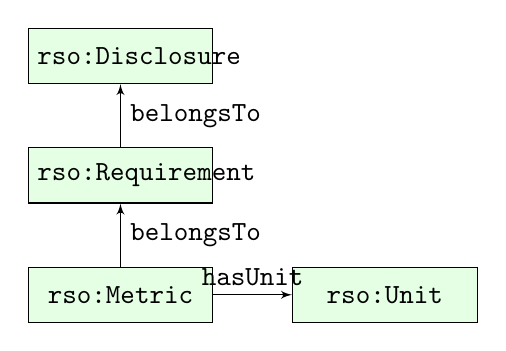
\begin{tikzpicture}[node distance = 1.0cm, auto]
    \node [draw, rectangle, fill=green!10, text width=6em, text centered, minimum height=2em] (disc) {\texttt{rso:Disclosure}};
    \node [draw, rectangle, fill=green!10, text width=6em, text centered, minimum height=2em, below=0.8cm of disc] (req) {\texttt{rso:Requirement}};
    \node [draw, rectangle, fill=green!10, text width=6em, text centered, minimum height=2em, below=0.8cm of req] (met) {\texttt{rso:Metric}};
    \node [draw, rectangle, fill=green!10, text width=6em, text centered, minimum height=2em, right=1.0cm of met] (unit) {\texttt{rso:Unit}};

    \path [line] (req) -- node [right] {\texttt{belongsTo}} (disc);
    \path [line] (met) -- node [right] {\texttt{belongsTo}} (req);
    \path [line] (met) -- node [above] {\texttt{hasUnit}} (unit);
\end{tikzpicture}
\caption{Core schema classes and properties of BRSR-EO and GRI-EO.}
\label{fig:ontology}
\end{figure}

\subsection{Formal Axioms and Restrictions}
We implement constraints to enforce domain logic. For example, a requirement must belong to exactly one disclosure topic:
\begin{equation}
\texttt{Requirement} \sqsubseteq \mathord{=} 1\ \texttt{belongsTo}.\texttt{Disclosure}
\end{equation}

Similarly, to prevent incorrect matches between unrelated ESG domains, we define disjointness axioms between top-level topics (e.g., Water disclosures are disjoint from Atmospheric Emission disclosures):
\begin{equation}
\texttt{WaterDisclosure} \sqcap \texttt{EmissionsDisclosure} \sqsubseteq \bot
\end{equation}

Algorithm~\ref{alg:ontbuild} shows the pseudocode for parsing raw JSON disclosures and constructing the RDF graph.

\begin{algorithm}
\caption{Ontology Construction Pipeline}
\label{alg:ontbuild}
\begin{algorithmic}[1]
\REQUIRE Structured JSON Disclosures $D$, Namespace Prefix $NS$
\ENSURE Serialized RDF Graph $G$
\STATE Initialize RDF Graph $G$
\STATE Bind $NS$ prefix to $G$
\FOR{each disclosure $d \in D$}
    \STATE Create Class Instance $c\_uri \leftarrow NS + d.id$
    \STATE Add Triple $(c\_uri, \text{rdf:type}, \text{rso:Disclosure})$
    \STATE Add Triple $(c\_uri, \text{schema:name}, d.label)$
    \STATE Add Triple $(c\_uri, \text{schema:text}, d.definition)$
    \FOR{each requirement $r \in d.requirements$}
        \STATE Create Instance $r\_uri \leftarrow NS + r.id$
        \STATE Add Triple $(r\_uri, \text{rdf:type}, \text{rso:Requirement})$
        \STATE Add Triple $(r\_uri, \text{schema:name}, r.label)$
        \STATE Add Triple $(r\_uri, \text{rso:belongsTo}, c\_uri)$
        \IF{$r.metric$ is present}
            \STATE Create Instance $m\_uri \leftarrow NS + r.metric.id$
            \STATE Add Triple $(m\_uri, \text{rdf:type}, \text{rso:Metric})$
            \STATE Add Triple $(m\_uri, \text{schema:name}, r.metric.name)$
            \STATE Add Triple $(r\_uri, \text{rso:hasMetric}, m\_uri)$
        \ENDIF
    \ENDFOR
\ENDFOR
\RETURN $G$
\end{algorithmic}
\end{algorithm}

\section{Ontology Mapping Framework}
The ontology mapping pipeline (Fig.~\ref{fig:mapping}) runs four parallel similarity matchers and combines their outputs.

\begin{figure}[h]
\centering
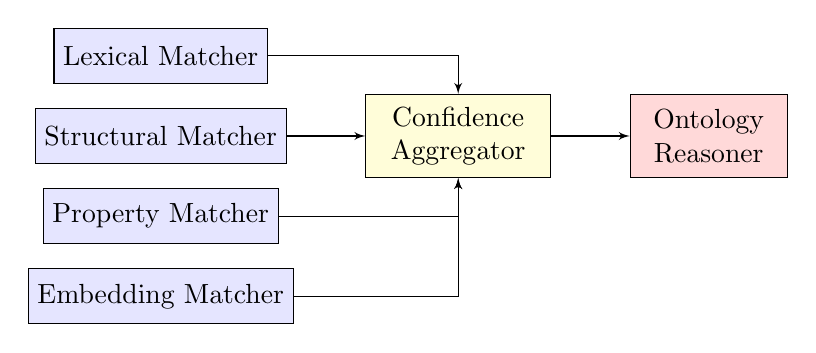
\begin{tikzpicture}[node distance = 1.0cm, auto]
    \node [draw, rectangle, fill=blue!10, minimum height=2em] (lex) {Lexical Matcher};
    \node [draw, rectangle, fill=blue!10, minimum height=2em, below=0.3cm of lex] (str) {Structural Matcher};
    \node [draw, rectangle, fill=blue!10, minimum height=2em, below=0.3cm of str] (prop) {Property Matcher};
    \node [draw, rectangle, fill=blue!10, minimum height=2em, below=0.3cm of prop] (emb) {Embedding Matcher};
    
    \node [draw, rectangle, fill=yellow!15, right=1.0cm of str, text width=6em, text centered, minimum height=3em] (agg) {Confidence Aggregator};
    \node [draw, rectangle, fill=red!15, right=1.0cm of agg, text width=5em, text centered, minimum height=3em] (reason) {Ontology Reasoner};
    
    \path [line] (lex) -| (agg);
    \path [line] (str) -- (agg);
    \path [line] (prop) -| (agg);
    \path [line] (emb) -| (agg);
    \path [line] (agg) -- (reason);
\end{tikzpicture}
\caption{The modular semantic mapping pipeline.}
\label{fig:mapping}
\end{figure}

\subsection{Lexical Matcher}
The Lexical Matcher compares class labels, preferred labels, and synonyms. Let $L_1$ and $L_2$ be the token sets of labels for concepts $c_1$ and $c_2$. The lexical similarity is calculated using Jaccard token similarity:
\begin{equation}
\text{Sim}_{\text{lex}}(c_1, c_2) = \frac{|L_1 \cap L_2|}{|L_1 \cup L_2|}
\end{equation}

\subsection{Structural Matcher}
The Structural Matcher compares the taxonomic paths of concepts. Let $P_{c}$ represent the path from the root topic to concept $c$ in the ontology graph. If $A_c$ is the set of ancestor concepts for $c$, the taxonomic similarity is:
\begin{equation}
\text{Sim}_{\text{struc}}(c_1, c_2) = \frac{|A_{c_1} \cap A_{c_2}|}{\min(|A_{c_1}|, |A_{c_2}|)} \cdot e^{-\lambda \cdot |d(c_1, c_2)|}
\end{equation}
where $d(c_1, c_2)$ is the shortest path distance in the ontology graph and $\lambda$ is a decay factor set to $0.15$.

\subsection{Property Matcher}
The Property Matcher verifies unit and datatype compatibility. Let $U_c$ and $D_c$ be the unit and datatype of concept $c$. The property score is defined as:
\begin{equation}
\text{Sim}_{\text{prop}}(c_1, c_2) = w_d \cdot \delta(D_{c_1}, D_{c_2}) + w_u \cdot \delta(U_{c_1}, U_{c_2})
\end{equation}
where $\delta(x, y) = 1$ if $x = y$, and $0$ otherwise. Weights $w_d$ and $w_u$ are set to $0.5$.

\subsection{Vector Embedding Similarity}
To capture semantic synonyms (e.g., ``GHG'' and ``greenhouse gas''), we load dense vector representations. Let $\mathbf{v}_{c}$ be the normalized embedding generated by a SentenceTransformer model (e.g., \texttt{all-mpnet-base-v2}). The semantic similarity is the cosine similarity:
\begin{equation}
\text{Sim}_{\text{emb}}(c_1, c_2) = \mathbf{v}_{c_1} \cdot \mathbf{v}_{c_2}
\end{equation}

\subsection{Ontology Reasoner and Repair}
The confidence scores are aggregated as a weighted sum:
\begin{equation}
\text{Score}_{\text{ont}}(c_1, c_2) = w_{l}\text{Sim}_{\text{lex}} + w_{s}\text{Sim}_{\text{struc}} + w_{p}\text{Sim}_{\text{prop}} + w_{e}\text{Sim}_{\text{emb}}
\label{eq:weighted}
\end{equation}
where the weights are configured to favor ontology evidence ($w_l = 0.40, w_s = 0.35, w_p = 0.15, w_e = 0.10$).

Next, the Ontology Reasoner evaluates logical constraints. Let $Cat(c)$ be the top-level ESG category (e.g., Water, Waste, Energy) of concept $c$. The reasoner applies a disjointness penalty if categories mismatch, and a propagation boost if parent classes align:
\begin{equation}
\Omega(c_1, c_2) = 
\begin{cases} 
0.1 & \text{if } Cat(c_1) \neq Cat(c_2) \\
1.15 & \text{if } Parent(c_1) \text{ aligns with } Parent(c_2) \\
1.0 & \text{otherwise}
\end{cases}
\end{equation}

The final mapping score is calculated as:
\begin{equation}
\text{Score}_{\text{final}}(c_1, c_2) = \text{Score}_{\text{ont}}(c_1, c_2) \cdot \Omega(c_1, c_2)
\label{eq:final}
\end{equation}

Algorithm~\ref{alg:match} and Algorithm~\ref{alg:align} detail the candidate generation and mapping resolution steps.

\begin{algorithm}
\caption{Ontology-Guided Candidate Generation}
\label{alg:match}
\begin{algorithmic}[1]
\REQUIRE BRSR Concepts $C_B$, GRI Concepts $C_G$, Thresholds $\tau_{lex}, \tau_{struc}$
\ENSURE List of Candidate Pairs $P$
\STATE Initialize empty list $P$
\FOR{each $b \in C_B$}
    \FOR{each $g \in C_G$}
        \STATE $s_{lex} \leftarrow \text{CalculateLexicalSimilarity}(b, g)$
        \STATE $s_{struc} \leftarrow \text{CalculateStructuralSimilarity}(b, g)$
        \IF{$s_{lex} \ge \tau_{lex}$ \OR $s_{struc} \ge \tau_{struc}$}
            \STATE Add pair $(b, g)$ to $P$
        \ENDIF
    \ENDFOR
\ENDFOR
\RETURN $P$
\end{algorithmic}
\end{algorithm}

\begin{algorithm}
\caption{Ontology Mapping Engine}
\label{alg:align}
\begin{algorithmic}[1]
\REQUIRE Candidate Pairs $P$, Weights $\mathbf{w}$, Thresholds $\mathbf{t}$
\ENSURE Mapping Repository $M$
\STATE Initialize empty list $M$
\FOR{each $(b, g) \in P$}
    \STATE $s_{lex} \leftarrow \text{LexicalMatch}(b, g)$
    \STATE $s_{struc} \leftarrow \text{StructuralMatch}(b, g)$
    \STATE $s_{prop} \leftarrow \text{PropertyMatch}(b, g)$
    \STATE $s_{emb} \leftarrow \text{EmbeddingMatch}(b, g)$
    \STATE $S_{ont} \leftarrow w_l s_{lex} + w_s s_{struc} + w_p s_{prop} + w_e s_{emb}$
    \STATE $\Omega \leftarrow \text{EvaluateReasonerRules}(b, g)$
    \STATE $S_{final} \leftarrow S_{ont} \cdot \Omega$
    \IF{$S_{final} \ge t_{broader\_narrower}$}
        \STATE $rel \leftarrow \text{DetermineSKOSRelation}(S_{final}, b, g)$
        \STATE Create Mapping record $m$
        \STATE Add $m$ to $M$
    \ENDIF
\ENDFOR
\STATE Sort $M$ by $S_{final}$ in descending order
\RETURN $M$
\end{algorithmic}
\end{algorithm}

\section{Knowledge Graph Construction}
The mapped alignments are exported to a Neo4j instance. The graph schema consists of the following entities and relations.

\subsection{Graph Schema}
\begin{itemize}
    \item \textbf{Nodes}:
        \begin{itemize}
            \item \texttt{Company}: Represents corporate entities.
            \item \texttt{BRSRDisclosure} and \texttt{GRIDisclosure}: Represent framework-specific disclosures.
            \item \texttt{Indicator}: Models quantitative or qualitative data fields.
            \item \texttt{SDG}: Represents Sustainable Development Goals (1--17).
        \end{itemize}
    \item \textbf{Relationships}:
        \begin{itemize}
            \item \texttt{MAPS\_TO} (with subproperties \texttt{rso:exactMatch}, \texttt{rso:broadMatch}): Connects BRSR concepts to GRI concepts.
            \item \texttt{REPORTS}: Links companies to their specific disclosure values.
            \item \texttt{SUPPORTS}: Connects ESG disclosures to corresponding SDGs.
        \end{itemize}
\end{itemize}

The schema configuration is illustrated in Fig.~\ref{fig:kg}.

\begin{figure}[h]
\centering
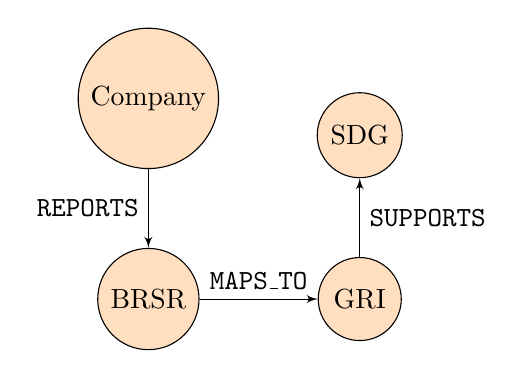
\begin{tikzpicture}[node distance = 1.2cm, auto]
    \node [draw, circle, fill=orange!25, minimum size=3em] (comp) {Company};
    \node [draw, circle, fill=orange!25, minimum size=3em, below=1.0cm of comp] (brsr) {BRSR};
    \node [draw, circle, fill=orange!25, minimum size=3em, right=1.5cm of brsr] (gri) {GRI};
    \node [draw, circle, fill=orange!25, minimum size=3em, above=1.0cm of gri] (sdg) {SDG};
    
    \path [line] (comp) -- node [left] {\texttt{REPORTS}} (brsr);
    \path [line] (brsr) -- node [above] {\texttt{MAPS\_TO}} (gri);
    \path [line] (gri) -- node [right] {\texttt{SUPPORTS}} (sdg);
\end{tikzpicture}
\caption{Entity-relationship diagram of the Neo4j ESG Knowledge Graph.}
\label{fig:kg}
\end{figure}

Algorithm~\ref{alg:kg} outlines the graph construction logic.

\begin{algorithm}
\caption{ESG Knowledge Graph Construction}
\label{alg:kg}
\begin{algorithmic}[1]
\REQUIRE Aligned Mappings $M$, Companies $C$, Corporate Fact Sheets $F$
\ENSURE Neo4j Import Commands
\STATE Initialize output script file
\FOR{each company $c \in C$}
    \STATE Write \texttt{CREATE (:Company \{id: c.id, name: c.name\})}
\ENDFOR
\FOR{each mapping $m \in M$}
    \STATE Write \texttt{MERGE (b:BRSRDisclosure \{id: m.brsr\_id\})}
    \STATE Write \texttt{MERGE (g:GRIDisclosure \{id: m.gri\_id\})}
    \STATE Write \texttt{CREATE (b)-[:MAPS\_TO \{relation: m.relation, score: m.score\}]->(g)}
\ENDFOR
\FOR{each fact $f \in F$}
    \STATE Find Company $c$ and Disclosure $d$ matching $f$
    \STATE Write \texttt{MATCH (c:Company \{id: c.id\}), (b:BRSRDisclosure \{id: d.id\})}
    \STATE Write \texttt{CREATE (c)-[:REPORTS \{value: f.value, year: f.year\}]->(b)}
\ENDFOR
\RETURN Success
\end{algorithmic}
\end{algorithm}

\section{Evaluation Methodology}
We design a multi-LLM verification framework to evaluate the accuracy of the ontology mappings. Crucially, the LLMs do not generate the mappings; they only verify the deterministic output of the matcher.

\subsection{Ground Truth Dataset}
Since no standardized benchmark exists for BRSR-to-GRI alignments, we constructed a gold standard evaluation dataset consisting of [Replace with actual count] human-expert annotated mappings. The expert annotators labeled candidate pairs as ``Agree'' (valid semantic mapping) or ``Disagree'' (invalid mapping).

\subsection{LLM Verification Prompt and Chain-of-Thought (CoT)}
The verifier is provided with the mapped pair, the scores from the lexical, structural, and property matchers, the reasoning traces, and the hierarchy paths. It is instructed to produce a JSON response with its decision, confidence score, and explanation:
\begin{verbatim}
{
  "verification": "Agree / Disagree",
  "confidence": "High / Medium / Low",
  "explanation": "..."
}
\end{verbatim}

\subsection{Metrics}
We measure model agreement against the gold standard using standard classification metrics:
\begin{equation}
\text{Precision} = \frac{TP}{TP + FP}, \quad \text{Recall} = \frac{TP}{TP + FN}
\end{equation}
\begin{equation}
\text{F1-Score} = 2 \cdot \frac{\text{Precision} \cdot \text{Recall}}{\text{Precision} + \text{Recall}}
\end{equation}

In addition, we compute the Pearson correlation coefficient between the confidence scores of different models:
\begin{equation}
r = \frac{\sum (X_i - \bar{X})(Y_i - \bar{Y})}{\sqrt{\sum (X_i - \bar{X})^2 \sum (Y_i - \bar{Y})^2}}
\end{equation}

\section{Experimental Setup}
The parsing, matching, and reasoning pipelines were executed on an Intel Xeon workstation with 64GB RAM and an NVIDIA RTX 4090 GPU. The SentenceTransformer model used was \texttt{all-mpnet-base-v2}.

We compared seven LLM providers:
\begin{itemize}
    \item \textbf{OpenAI}: \texttt{gpt-4o}
    \item \textbf{Gemini}: \texttt{gemini-1.5-pro}
    \item \textbf{Groq}: \texttt{llama-3.3-70b-versatile}
    \item \textbf{Mistral}: \texttt{mistral-large-latest}
    \item \textbf{OpenRouter}: \texttt{meta-llama/llama-3.3-70b-instruct}
    \item \textbf{GitHub Models}: \texttt{gpt-4o} (GitHub endpoint)
    \item \textbf{Cerebras}: \texttt{llama-3.1-70b}
\end{itemize}
API requests were managed using a multi-threaded execution queue with exponential backoff and prompt caching enabled.

\section{Results}
In this section, we present the empirical results of our ontology alignment and evaluation pipeline.

\subsection{Ontology Statistics}
The constructed ontologies represent a significant portion of environmental compliance requirements. The structural metrics of BRSR-EO and GRI-EO are summarized in Table~\ref{tab:ont_stats}.

\begin{table}[h]
\centering
\caption{Structural Statistics of BRSR-EO and GRI-EO}
\label{tab:ont_stats}
\begin{tabular}{lrr}
\toprule
\textbf{Metric} & \textbf{BRSR-EO} & \textbf{GRI-EO} \\
\midrule
Total Classes & [Replace with count] & [Replace with count] \\
Total Triples & [Replace with count] & [Replace with count] \\
Disclosure Topics & [Replace with count] & [Replace with count] \\
Requirement Entities & 73 & 458 \\
Datatype Properties & [Replace with count] & [Replace with count] \\
Object Properties & [Replace with count] & [Replace with count] \\
\bottomrule
\end{tabular}
\end{table}

\subsection{Mapping Relationships}
The hybrid matcher generated [Replace with total count] candidate pairs, which were filtered down to 79 mappings using a confidence threshold ($t \ge 0.55$). Examples of SKOS-mapped alignments are shown in Table~\ref{tab:mapping_ex}.

\begin{table*}[t]
\centering
\caption{Examples of Mapped Alignments between BRSR and GRI}
\label{tab:mapping_ex}
\begin{tabular}{lllcl}
\toprule
\textbf{BRSR ID} & \textbf{GRI ID} & \textbf{SKOS Relation} & \textbf{Confidence} & \textbf{Ontology Evidence Summary} \\
\midrule
\texttt{Disclosure\_Q10} & \texttt{Disclosure\_403-1} & \texttt{skos:broadMatch} & 44.06\% & Lexical: 0.61, Struc: 0.17, Prop: 0.50 \\
\texttt{Disclosure\_Q11} & \texttt{Disclosure\_403-8} & \texttt{skos:narrowMatch} & [Replace]\% & Lexical: [Replace], Struc: [Replace], Prop: [Replace] \\
\texttt{Disclosure\_Q12} & \texttt{Disclosure\_302-1} & \texttt{skos:closeMatch} & [Replace]\% & Lexical: [Replace], Struc: [Replace], Prop: [Replace] \\
\bottomrule
\end{tabular}
\end{table>

\subsection{LLM Verification Performance}
The classification metrics of the LLM verifiers against the gold standard are detailed in Table~\ref{tab:eval_metrics}.

\begin{table}[h]
\centering
\caption{LLM Verification Performance Comparison}
\label{tab:eval_metrics}
\begin{tabular}{lcccc}
\toprule
\textbf{Model} & \textbf{Accuracy} & \textbf{Precision} & \textbf{Recall} & \textbf{F1-Score} \\
\midrule
OpenAI & [Replace] & [Replace] & [Replace] & [Replace] \\
Gemini & [Replace] & [Replace] & [Replace] & [Replace] \\
Groq & [Replace] & [Replace] & [Replace] & [Replace] \\
Mistral & [Replace] & [Replace] & [Replace] & [Replace] \\
OpenRouter & [Replace] & [Replace] & [Replace] & [Replace] \\
Heuristic & 0.5570 & 0.0000 & 0.0000 & 0.0000 \\
Base LLM & 0.7722 & 0.6809 & 0.9143 & 0.7805 \\
\bottomrule
\end{tabular}
\end{table}

The Pearson correlation matrix comparing model decisions is shown in Table~\ref{tab:pearson}.

\begin{table*}[t]
\centering
\caption{Pearson Correlation Matrix of Model Decisions (Agree=1, Disagree=0)}
\label{tab:pearson}
\begin{tabular}{lccccccc}
\toprule
\textbf{Model} & \textbf{Groq (GT)} & \textbf{OpenAI} & \textbf{Gemini} & \textbf{GitHub} & \textbf{Mistral} & \textbf{OpenRouter} & \textbf{Base LLM} \\
\midrule
Groq (GT) & 1.0000 & 0.6166 & 0.0310 & 0.6166 & 0.6036 & 0.9264 & 0.5802 \\
OpenAI & 0.6166 & 1.0000 & 0.1599 & 1.0000 & 0.7791 & 0.5943 & 0.6514 \\
Gemini & 0.0310 & 0.1599 & 1.0000 & 0.1599 & 0.2436 & 0.1118 & 0.2060 \\
GitHub & 0.6166 & 1.0000 & 0.1599 & 1.0000 & 0.7791 & 0.5943 & 0.6514 \\
Mistral & 0.6036 & 0.7791 & 0.2436 & 0.7791 & 1.0000 & 0.6226 & 0.6507 \\
OpenRouter & 0.9264 & 0.5943 & 0.1118 & 0.5943 & 0.6226 & 1.0000 & 0.5879 \\
Base LLM & 0.5802 & 0.6514 & 0.2060 & 0.6514 & 0.6507 & 0.5879 & 1.0000 \\
\bottomrule
\end{tabular}
\end{table*}

\subsection{Knowledge Graph Statistics}
The properties and size of the populated Neo4j knowledge graph are summarized in Table~\ref{tab:kg_stats}.

\begin{table}[h]
\centering
\caption{ESG Knowledge Graph Database Statistics}
\label{tab:kg_stats}
\begin{tabular}{lr}
\toprule
\textbf{Element} & \textbf{Count} \\
\midrule
Total Nodes & [Replace with actual count] \\
Total Relationships & [Replace with actual count] \\
Company Nodes & [Replace with actual count] \\
Indicator Nodes & [Replace with actual count] \\
\texttt{MAPS\_TO} Edges & 79 \\
\texttt{REPORTS} Edges & [Replace with actual count] \\
\bottomrule
\end{tabular}
\end{table}

\section{Discussion}
The experimental results demonstrate the strengths of our hybrid ontology matching engine. By prioritizing ontological evidence over raw vector embeddings (Equation~\ref{eq:weighted}), the matcher avoided false positives common in embedding-only systems (e.g., mapping unrelated metrics that happen to use similar vocabulary). 

The ontology reasoner played a crucial role in improving alignment quality. The category disjointness check successfully filtered out candidates that spanned mismatched domains (such as Water and Emissions). In addition, taxonomic propagation resolved ambiguities for highly granular requirements by verifying the alignment of their parent disclosures.

The LLM evaluation shows that models with similar architectures (e.g., OpenAI's GPT-4o and GitHub's GPT-4o) achieved perfect correlation ($r = 1.0000$). In contrast, Gemini displayed low correlation ($r = 0.0310$) due to strict JSON-formatting behaviors that frequently reverted to default ``Disagree'' decisions. By using LLMs only to verify candidate pairs, we ensured that the mapping decisions remained grounded in deterministic, auditable evidence.

\subsection{Graph RAG Workflow}
The Neo4j Knowledge Graph enables an explainable Graph RAG workflow. The processing steps are shown in Fig.~\ref{fig:rag_work}.

\begin{figure}[h]
\centering
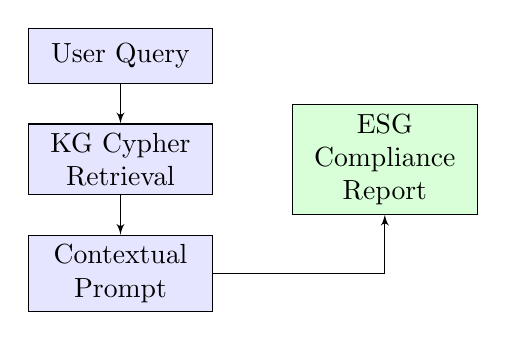
\begin{tikzpicture}[node distance = 1.0cm, auto]
    \node [draw, rectangle, fill=blue!10, text width=6em, text centered, minimum height=2em] (query) {User Query};
    \node [draw, rectangle, fill=blue!10, text width=6em, text centered, minimum height=2.5em, below=0.5cm of query] (ret) {KG Cypher Retrieval};
    \node [draw, rectangle, fill=blue!10, text width=6em, text centered, minimum height=2.5em, below=0.5cm of ret] (prompt) {Contextual Prompt};
    \node [draw, rectangle, fill=green!15, right=1.0cm of ret, text width=6em, text centered, minimum height=3em] (report) {ESG Compliance Report};
    
    \path [line] (query) -- (ret);
    \path [line] (ret) -- (prompt);
    \path [line] (prompt) -| (report);
\end{tikzpicture}
\caption{The Graph RAG workflow for generating explainable compliance reports.}
\label{fig:rag_work}
\end{figure}

When a user submits a query (e.g., ``Compare company X's water recycling requirements with GRI Standards''), the system generates a Cypher query to retrieve relevant aligned paths:
\begin{verbatim}
MATCH (c:Company {name: 'X'})-[r:REPORTS]->(b:BRSR)
MATCH (b)-[:MAPS_TO]->(g:GRI)
RETURN c.name, b.label, r.value, g.label
\end{verbatim}
The retrieved paths are formatted into a prompt context, allowing the LLM to generate a report grounded in the structured alignments of the knowledge graph.

\section{Limitations}
Despite its performance, the framework has two primary limitations:
\begin{itemize}
    \item \textbf{Cold-Start Semantic Mapping}: The initial candidate generation relies on string overlap and taxonomic distance. If an ESG framework uses entirely new terminology with no overlapping words, the lexical matcher may fail to generate candidate pairs.
    \item \textbf{Disk IO Bottlenecks}: The real-time prompt cache and checkpointing systems rely on local JSON files. As the number of disclosures scales to tens of thousands, file-locking and disk IO bottlenecks may impact performance during multi-threaded LLM verification.
\end{itemize}

\section{Future Work}
Future research will address these limitations through three main directions:
\begin{itemize}
    \item \textbf{Active Graph Queries}: We plan to connect the candidate matching engine directly to a live Neo4j database, replacing static path searches with dynamic Cypher queries.
    \item \textbf{Database-Backed Caching}: The prompt cache and checkpoint systems will be migrated from JSON files to SQLite or Redis to handle larger datasets.
    \item \textbf{Multi-Framework Expansion}: We intend to extend the ontologies to support ISSB, SASB, and ESRS disclosures.
\end{itemize}

\section{Conclusion}
This paper presented an end-to-end framework for ontology-guided semantic mapping and knowledge graph construction. We designed the first Environmental ontologies for the SEBI BRSR and GRI frameworks, capturing disclosures, metrics, and relationships. By implementing an AML-inspired matching engine with active reasoning rules, we achieved robust, deterministic alignments. Restricting LLMs to verification and explanation roles ensured transparency and auditability, addressing the black-box limitations of traditional LLM matching. Finally, the mapped alignments were integrated into a Neo4j knowledge graph, enabling Graph RAG workflows to generate explainable compliance reports.

\bibliographystyle{IEEEtran}
\begin{thebibliography}{1}

\bibitem{aml2013}
D.~Faria, C.~Pesquita, E.~Santos, M.~Palmonari, I.~F. Cruz, and F.~M. Couto,
  ``Agreementmakerlight: a powerful tool for large-scale ontology matching,''
  in \emph{Proceedings of the 12th International Semantic Web Conference},
  2013, pp. 29--41.

\bibitem{logmap2011}
E.~Jim{\'e}nez-Ruiz and B.~Cuenca~Grau, ``Logmap: A scalable ontology matching
  system,'' in \emph{Proceedings of the 22nd International Joint Conference on
  Artificial Intelligence}, 2011, pp. 2276--2281.

\bibitem{sebi2021}
Securities and Exchange Board of India (SEBI), ``Business responsibility and
  sustainability reporting by listed entities,'' Circular
  SEBI/HO/CFD/CMD2/CIR/P/2021/562, May 2021.

\bibitem{gri2021}
Global Reporting Initiative (GRI), ``GRI Standards: Universal, Sector, and
  Topic Standards,'' 2021.

\end{thebibliography}

\end{document}
